\pdfoutput=1
% CVPR 2025 Paper Template; see https://github.com/cvpr-org/author-kit

\documentclass[10pt,twocolumn,letterpaper,dvipsnames,table]{article}

%%%%%%%%% PAPER TYPE  - PLEASE UPDATE FOR FINAL VERSION
\usepackage{cvpr}              % To produce the CAMERA-READY version
%\usepackage{pdfpages}
% \usepackage[review]{cvpr}      % To produce the REVIEW version
% \usepackage[pagenumbers]{cvpr} % To force page numbers, e.g. for an arXiv version
\usepackage{makecell}
\usepackage{amssymb} % 引入宏包以使用对号和错号
\usepackage[accsupp]{axessibility}  % Improves PDF readability for those with disabilities.
% Import additional packages in the preamble file, before hyperref
%
% --- inline annotations
%
\newcommand{\red}[1]{{\color{red}#1}}
\newcommand{\todo}[1]{{\color{red}#1}}
\newcommand{\TODO}[1]{\textbf{\color{red}[TODO: #1]}}
% --- disable by uncommenting  
% \renewcommand{\TODO}[1]{}
% \renewcommand{\todo}[1]{#1}



% It is strongly recommended to use hyperref, especially for the review version.
% hyperref with option pagebackref eases the reviewers' job.
% Please disable hyperref *only* if you encounter grave issues, 
% e.g. with the file validation for the camera-ready version.
%
% If you comment hyperref and then uncomment it, you should delete *.aux before re-running LaTeX.
% (Or just hit 'q' on the first LaTeX run, let it finish, and you should be clear).
\definecolor{cvprblue}{rgb}{0.21,0.49,0.74}
% \usepackage[pagebackref,breaklinks,colorlinks,allcolors=cvprblue]{hyperref}

% According to https://www.overleaf.com/learn/how-to/LaTeX_checklist_for_arXiv_submissions
\usepackage{hyperref}
\hypersetup{pagebackref,breaklinks,colorlinks,allcolors=cvprblue}


%%%%%%%%% PAPER ID  - PLEASE UPDATE
\def\paperID{8339} % *** Enter the Paper ID here
\def\confName{CVPR}
\def\confYear{2025}

%%%%%%%%% TITLE - PLEASE UPDATE
\title{AdaMMS: Model Merging  for Heterogeneous Multimodal Large Language Models with Unsupervised Coefficient Optimization }

%%%%%%%%% AUTHORS - PLEASE UPDATE
% \author{First Author\\
% Institution1\\
% Institution1 address\\
% {\tt\small firstauthor@i1.org}
% % For a paper whose authors are all at the same institution,
% % omit the following lines up until the closing ``}''.
% % Additional authors and addresses can be added with ``\and'',
% % just like the second author.
% % To save space, use either the email address or home page, not both
% \and
% Second Author\\
% Institution2\\
% First line of institution2 address\\
% {\tt\small secondauthor@i2.org}
% }

\author{
Yiyang Du\textsuperscript{*,1}, 
Xiaochen Wang\textsuperscript{*,3,4}, 
Chi Chen\textsuperscript{*,1}, 
Jiabo Ye\textsuperscript{5},
Yiru Wang\textsuperscript{8}, \\ 
{
Peng Li \textsuperscript{\Letter,2,6}, 
Ming Yan\textsuperscript{5}, 
Ji Zhang\textsuperscript{5}, 
Fei Huang\textsuperscript{5}, 
Zhifang Sui\textsuperscript{3}, 
Maosong Sun\textsuperscript{1}, 
Yang Liu\textsuperscript{\Letter,1,2,6,7}} \\
  \textsuperscript{1}Dept. of Comp. Sci. \& Tech., Institute for AI, Tsinghua University, Beijing, China \\
  \textsuperscript{2}Institute for AI Industry Research (AIR), Tsinghua University, Beijing, China \\
  \textsuperscript{3}State Key Laboratory of Multimedia Information Processing, Peking University, Beijing, China\\
  \textsuperscript{4}School of Software Microelectronics, Peking University, Beijing, China\\
  \textsuperscript{5}Institute of Intelligent Computing, Alibaba Group\\
  \textsuperscript{6}Shanghai Artificial Intelligence Laboratory, Shanghai, China\\
  \textsuperscript{7}Jiangsu Collaborative Innovation Center for Language Competence, Jiangsu, China\\
  \textsuperscript{8}ModelTC Open Source Organization, Beijing, China
}

\begin{document}
\maketitle
\begin{abstract}
Fine-tuning provides an effective means to specialize pre-trained models for various downstream tasks. However, fine-tuning often incurs high memory overhead, especially for large transformer-based models, such as LLMs. While existing methods may reduce certain parts of the memory required for fine-tuning, they still require caching all intermediate activations computed in the forward pass to update weights during the backward pass. In~this work, we develop \method, a method to reduce memory usage,  specifically the memory to store intermediate activations, in the fine-tuning of transformer-based models. During the backward pass, \method approximates the gradient computation by backpropagating through just a subset of input tokens. Thus, with \method, only a subset of intermediate activations are cached during the forward pass. Also, \method can be easily combined with existing methods like LoRA, further reducing the memory cost. We evaluate our approach on pre-trained transformer models with up to billions of parameters, considering the performance on multiple downstream tasks such as text classification and question answering in a few-shot learning setup. Overall, \method achieves performance on par with full fine-tuning or representative memory-efficient fine-tuning methods,  while greatly reducing the memory footprint, especially when combined with other methods with complementary memory reduction mechanisms. We hope that our approach will facilitate the fine-tuning of large transformers,  in specializing them for specific domains or co-training them with other neural components from a larger system. Our code is available at \githubURL.
\blfootnote{\textbf{*} Equal contribution}
\end{abstract}
    
\section{Introduction}
\label{sec:intro}

\begin{figure*}[t!]
    \centering
    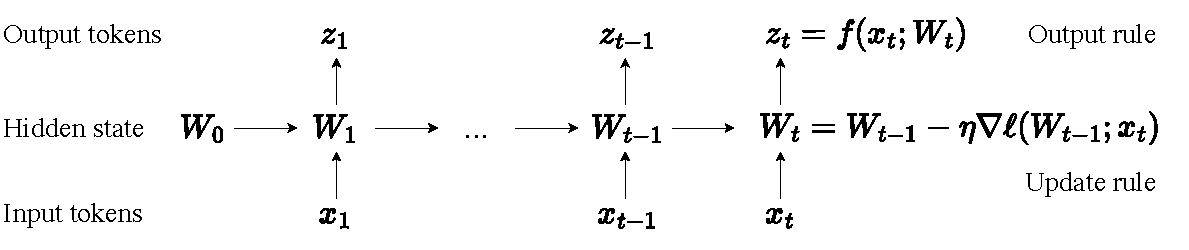
\includegraphics[width=0.8\textwidth]{figs/simple_teaser.pdf}
    \caption{All RNN layers can be expressed as a hidden state that transitions according to an update rule.
    The key idea in \cite{sun2024ttt} is to make the hidden state itself a model $f$ with weights $W$, and the update rule a gradient step on the self-supervised loss $\ell$.
    Therefore, updating the hidden state on a test sequence is equivalent to training the model $f$ at test time. 
    This process, known as Test-Time Training (TTT), is programmed into TTT layers. 
    Figure and caption taken from \cite{sun2024ttt}.
    }
    \label{fig:ttt-layer}
\end{figure*}

Despite the remarkable progress in visual and physical realism, state-of-the-art video Transformers are still generating mostly short clips of single scenes without complex stories.
At the time of writing (March 2025), the maximum length of public APIs for video generation is 20 seconds for Sora (OpenAI), 16 seconds for MovieGen (Meta), 10 for Ray~2 (Luma), and 8 for Veo~2 (Google).
None of these APIs can autonomously generate complex multi-scene stories.

A fundamental challenge behind these technical limitations is long context, because the cost of self-attention layers in Transformers increases quadratically with context length.
This challenge is especially acute for video generation with dynamic motion, whose context cannot be easily compressed by a tokenizer.
Using a standard tokenizer, each of our one-minute videos requires over 300k tokens in context. 
With self-attention, generating a one-minute video would have taken $11\times$ longer than generating 20 videos of 3 seconds each, and training would have taken $12\times$ longer.

To address this challenge, recent work on video generation has investigated RNN layers as an efficient alternative to self-attention, because their cost increases linearly with context length~\cite{wang2024lingenhighresolutionminutelengthtexttovideo}.
Modern RNN layers, especially variants of linear attention~\cite{schmidhuberlinearattn, katharopoulos2020lineartransformers} such as Mamba~\cite{gu2024mamba, dao2024mamba2} and DeltaNet~\cite{schlag2021deltanet, yang2025gateddeltanetworksimproving}, have shown impressive results for natural language tasks.
However, we have yet to see long videos with complex stories or dynamic motion generated by RNNs.
Videos (\href{https://lineargen.github.io/}{link}) in \cite{wang2024lingenhighresolutionminutelengthtexttovideo} are high resolution and one-minute long, but contain only single scenes and slow motion, let alone complex stories.

We believe that these RNN layers generate less complex videos because their hidden states are less expressive.
RNN layers can only store past tokens into a hidden state of fixed size, which is only a matrix for linear attention variants such as Mamba and DeltaNet.
It is inherently challenging to compress hundreds of thousands of vectors into a matrix with only thousands in rank.
As a consequence, these RNN layers struggle to remember the deep relationships between distant tokens.

We experiment with an alternative class of RNN layers whose hidden states themselves can be neural networks. Specifically, we use two-layer MLPs with 2$\times$ more hidden cells and richer nonlinearities than the linear (matrix) hidden states in linear attention variants.
Since the neural network hidden states are updated by training even on test sequences, these new layers are called Test-Time Training (TTT) layers~\cite{sun2024ttt}.

We start from a pre-trained Diffusion Transformer (CogVideo-X 5B \cite{hong2023cogvideo}) that could only generate 3-second short clips at 16 fps (or 6 seconds at 8 fps).
Then, we add TTT layers initialized from scratch and fine-tune this model to generate one-minute videos from text storyboards. 
We limit the self-attention layers to 3-second segments so their cost stays manageable.
With only preliminary systems optimization, our training run takes the equivalent of 50 hours on 256 H100s.

We curate a text-to-video dataset based on $\approx$ 7 hours of \textit{Tom and Jerry} cartoons with human-annotated storyboards.
We intentionally limit our scope to this specific domain for fast research iteration.
As a proof-of-concept, our dataset emphasizes complex, multi-scene, and long-range stories with dynamic motion, where progress is still needed; it has less emphasis on visual and physical realism, where remarkable progress has already been made.
We believe that improvements in long-context capabilities for this specific domain will transfer to general-purpose video generation.

Compared to strong baselines such as Mamba 2~\cite{dao2024mamba2}, Gated DeltaNet~\cite{yang2025gateddeltanetworksimproving}, and sliding-window attention layers, TTT layers generate much more coherent videos that tell complex stories with dynamic motion, leading by 34 Elo points in a human evaluation of 100 videos per method.
For context, GPT-4o scores 29 Elo points over GPT-4 Turbo in LMSys Chatbot Arena~\cite{chiang2024chatbot}.

Sample videos, code and annotations are available at:
\url{https://test-time-training.github.io/video-dit}
\section{Related Work}
\label{sec:bk}

\subsection{Model Merging}

Recent researches on model merging techniques have contributed to building more capable models by providing an efficient approach to combine abilities on various tasks from different models that requires less data and compute.
Some studies focus on merging homogeneous models with identical architecture, while others focus on tackle the challenge on heterogeneous models which have different architectures.
In merging homogeneous models, Task Arithmetic \cite{task-arithmetic} proposes the concept of task vectors, which subtracts fine-tuned weights from pre-train weights to obtain task-related weight difference as the object of merging. Ties-Merging \cite{ties} and DARE \cite{dare} further improve the performance by mitigating parameter interference during the merging process through parameter pruning and conflict resolving. MetaGPT \cite{metagpt} scales the task vectors with task-agnostic coefficients in closed-form by seperating data term and scaling coefficients in the optimization objective. Although these methods improves the performance of the merged models, they cannot be directly applied on models with architecture difference.
% Learnable-MAM \cite{sundar2024multimodalattentionmergingimproved}
In fusing heterogeneous models, DAMC \cite{modelcompose} employs parameter decoupling and adaptive adjustment to enhance model merging strategies for fusing modalities on MLLMs with different modality encoders, but this work still focus on merging identical language model architecture. To consolidate LLMs with different architectures, FuseLLM \cite{fusellm} and FuseChat \cite{fusechat} applies token alignment and model fusion strategies with knowledge distillation before continue training the model, but they need labeled data and computation resources for continue training.
In fact, the majority of previous works on model merging requires labeled data for validation search or supervised training \cite{task-arithmetic, ties, dare, modelcompose, fusellm, fusechat}. In this work, we eliminate the need of labeled data by leveraging our unsupervised hyper-parameter selection method, and enable model merging strategies to be applied on heterogeneous MLLMs with architecture differences.

%[TODO: previous ones?]. 
% Task Arithmetic \cite{task-arithmetic} proposes the concept of task vectors, which subtracts fine-tuned weights from pre-train weights to obtain task-related weight difference as the object of merging. To further improve the performance of the merged model, TIES-Merging \cite{ties} addresses parameter interference by dropping parameters with low magnitude and resolving sign conflicts, and DARE \cite{dare} applies random dropping and rescale to get rid of redundant parameters. MetaGPT \cite{metagpt} scales the task vectors with task-agnostic coefficients in closed-form by seperating data term and scaling coefficients in the optimization objective.
% With these model merging techniques, Sundar et. al combines knowledge to improve model performance on speech recognition tasks, DAMC \cite{modelcompose} additionally employs parameter decoupling and adaptive adjustment strategies to integrate multiple modalities. To consolidate LLMs with different architectures, FuseLLM \cite{fusellm} and FuseChat \cite{fusechat} applies token alignment and model fusion strategies with knowledge distillation before continue training the model. Our work follows the previous path of model merging techniques, and enables model merging to be applied on heterogeneous MLLMs with a superior performance.

\subsection{Multimodal Large Language Models} \label{mllms}

As large language models demonstrate huge success in obtaining great abilities in general, recent researches on MLLMs have successfully appending multimodal processing and generation ability on LLMs, especially on the vision modality \cite{llava1.5, sharegpt4v, mplugowl2, cogvlm, qwen2-vl, llava-onevison}. However, these models often adapts unique modifications on language model architecture, resulting in a set of heterogeneous MLLMs, which prevent model merging methods to be applied on them. Specifically, there are two levels of architecture differences among MLLMs. 
First, two MLLMs may be designed from different pre-trained language model. For example, Qwen2-VL \cite{qwen2-vl} and LLaVA-OneVision-Qwen \cite{llava-onevison} are designed from Qwen2 \cite{qwen2}, while LLaVA \cite{llava1.5}, mPLUG-Owl2 \cite{mplugowl2}, CogVLM \cite{cogvlm} and ShareGPT4V \cite{sharegpt4v} are designed following the LLaMA \cite{llama} architecture. 
Second, two MLLMs developed from the same pre-trained language model can still be heterogeneous because they are designed with different modifications on the language model. For example, although CogVLM and mPLUG-Owl2 are both developed from LLaMA architecture, CogVLM adapts visual experts by duplicating query, key and value weights in attention head, while mPLUG-Owl2 is designed to duplicate key, value, and layer norm weights instead. 
The first level of differences is hard to merge, since model merging applies to parameters that are trained from the same pre-training weights \cite{task-arithmetic}. In this work, we tackle the second level of architecture differences via our proposed \ours method.


% LLaVA-v1.5 \cite{llava1.5} connects vision encoder and LLM with an MLP projection, and the end-to-end MLLM is trained on massive multimodal datasets. Following this design, mPLUG-Owl2 \cite{mplugowl2} introduces a modality-adaptive module for self-attention block to improve the modality collaboration between vision and language. CogVLM \cite{cogvlm} adds a trainable visual expert to the language model in each layer to enable deep visual-language feature alignment. Qwen2-VL \cite{qwen2-vl} enables the model to dynamically process images of varying resolutions into different numbers of visual tokens through the Naive Dynamic Resolution mechanism. ShareGPT4V \cite{sharegpt4v} and LLaVA-OneVision \cite{llava-onevison} also push the frontier of vision MLLMs with better training data and vision encoders. Although there are many open-source MLLMs with powerful language and vision capabilities, combining their abilities through model merging technique faces great challenges for their inherent heterogeneous property due to their differences in language model architecture and vision encoder choice. Our proposed model merging technique alleviates these challenges and produces MLLMs with performance improvements on various vision-language tasks.
\section{Methodology}
\vspace{-5pt}


In this section, we introduce our formulation formally and present \ours for solving the alignment problem by optimizing the alignment instruction.

%Most existing methods for alignment use techniques like PPO \cite{Schulman2017ProximalPO} and DPO \cite{rafailov2023direct} which are very costly to execute as they need large amounts of data to be successful. 

% Most existing alignment methods, such as RLHF~\cite{ouyang2022training} and DPO~\cite{rafailov2023direct}, are generally expensive to execute, requiring not only large amounts of data but also substantial computational resources and human labeling efforts.
% Research on using in-context learning for alignment has been limited and primarily relies on human-generated prompts and in-context learning examples. To address this limitation, we introduce a systematic method to optimize prompts and in-context learning examples for LLMs without any human effort or annotation.


\subsection{Problem Formulation}

% \noindent \textbf{Problem Formulation}.
Given an LLM $\mathcal{B}$, an alignment instruction consists of two parts: a system prompt $\mathcal{P}$ and a set of $N$ in-context learning (ICL) examples $\mathcal{I}$.
The system prompt $\mathcal{P}$ serves as a prefix that provides high-level instructions, sets the tone, and imposes constraints on the model's responses. Each ICL example $\mathcal{I}_i$ consists of a pair $(q_i, d_i)$, where $q_i$ is an input query and $d_i$ is the corresponding desired response, so we can represent $\mathcal{I} = \{(q_1, d_1), (q_2, d_2), \ldots, (q_N, d_N)\}$. 

Conditioning on the system prompt $\mathcal{P}$ and a selected subset of $K$ ICL examples $\mathcal{I}_K \subseteq \mathcal{I}$, the aligned model response $y$ to an input $x$ is generated as:
\[
y = \mathcal{B}(x \mid \mathcal{P}, \mathcal{I}_K)
\]

\ours aims to optimize both system prompt $\mathcal{P}$ and ICL examples $\mathcal{I}_K$ to enhance alignment. This involves finding the best possible $\mathcal{P}^*$ and $\mathcal{I}_K^*$ that maximize the alignment of the model's responses. This optimization problem can be formulated as follows:
\[
(\mathcal{P}^*, \mathcal{I}_K^*) = \arg\max_{\mathcal{P}, \mathcal{I}_K} \mathbb{E}_{x \sim \mathcal{D}_x} \left[\mathcal{B}(x \mid \mathcal{P}, \mathcal{I}_K) \right]
\]
\noindent where $\mathcal{D}_x$ denotes the distribution of input queries, and the expectation $\mathbb{E}$ represents the alignment performance for responses based on specific metrics.


% We propose a two-step approach to the optimization problem: 
% \begin{enumerate}
%     \item Estimating $\mathcal{I}^*$ (universal).
%     \item Estimating $\mathcal{P}^*$ given ${\mathcal{I}}^*$. (model specific)
% \end{enumerate}


% \subsection{Systematic Optimization Framework}

% We approach the optimization of the system prompt $\mathcal{P}$ and in-context learning examples $\mathcal{E}$ using the unified framework LLM Reasoners~\cite{hao2024llm} that involves a base model $\mathcal{B}$, an optimizer $\mathcal{O}$, and an evaluator $\mathcal{E}$. This framework is treated as a search process that iteratively interacts with the model's environment and adjusts the prompt $\mathcal{P}$ based on a reward function $\mathcal{R}$. The main challenge for our problem is -the design of a reward function for a problem as broad and general as Alignment. To overcome this challenge we introduce `Dynamic Rewarding', which can effectively handle tasks as broad and challenging as alignment.


\subsection{Dynamic Rewarding with Prompt Optimization (\ours)}

Given the distinct nature of the system prompt and ICL examples, we propose to optimize them separately, resulting in a two-step optimization approach. We first construct a universal set of ICL examples and optimize their responses to obtain $\mathcal{I}^*$. Next, we estimate a model-specific system prompt $\mathcal{P}^*$ based on the optimized universal set $\mathcal{I}^*$. Notably, we leverage the \texttt{LLM Reasoners}\footnote{\url{https://github.com/maitrix-org/llm-reasoners}} framework~\cite{hao2023reasoning, hao2024llm} as the prompt optimization (PO) framework. Specifically, \texttt{LLM Reasoners} incorporates a base model $\mathcal{B}$, an optimizer $\mathcal{O}$, and an evaluator $\mathcal{E}$. It operates as a search agent that iteratively interacts with the model's environment, using the optimizer $\mathcal{O}$ to adjust the prompt $\mathcal{P}$ or ICL examples $\mathcal{I}$ based on a reward function $\mathcal{R}$. For further details, we refer readers to the original references. In the following, we introduce the core component of \ours. 


\subsubsection{Dynamic Rewarding for Alignment}

We formulate this optimization problem as a Markov Decision Process (MDP). In this framework, the states $s\in \mathcal{S}$ represent our optimization goal, which could be either a system prompt or an in-context example. Actions $a \in \mathcal{A}$ are defined based on the alignment feedback obtained during the evaluation of any given state. The key motivation is to leverage the superior generalization capabilities of LLMs to evaluate and analyze states, guiding state transitions toward an optimal state. We employ different evaluation techniques for system prompt and in-context example optimization, which are detailed in subsequent sections. Efficient traversal of this state space is crucial, and for this purpose, we adopt beam search due to its effectiveness and low computational cost.


One of the key challenges in our optimization task is designing a reward function capable of handling a problem as broad and generalized as alignment. As illustrated in Figure~\ref{fig:dynamic_rewarding}, a single, unified reward function is impractical due to the vast query space we aim to align with the base LLM $\mathcal{B}$. Different queries emphasize different focal points, meaning that certain evaluation criteria might be appropriate for some queries but not for others. To overcome this, we introduce a dynamic reward function $\mathcal{R}$, which can dynamically adapt to the specific query being evaluated. Notably, our approach shares conceptual similarities with a few recent alignment research, which also advocate for adaptable and query-sensitive alignment strategies~\cite{bai2022constitutional, sun2024principle}. However, the key distinction lies in our dynamic reward function’s ability to not only enable flexible evaluation but also integrate seamlessly into a formally defined optimization framework.



Specifically, we first predefined a set of reward criteria $\mathbb{R}$, from which the model dynamically selects the most relevant rewards, while also retaining the flexibility to propose new ones when necessary. Formally, for a given query \( q \), the dynamic reward function $\mathcal{R}$ evaluates the model's response $\sigma$ based on a dynamically selected or proposed rewards $\mathbb{R}_q$, where $\mathbb{R}_q \subseteq \mathbb{R} \cup \mathbb{R}^*$ and $\mathbb{R}^*$ represents newly proposed rewards. The reward function is defined as:

\[
\mathcal{R}(\sigma \mid \mathbb{R}_q) = \frac{1}{|\mathbb{R}_q|} \sum_{r \in \mathbb{R}_q} r(\sigma)
\]

Here, $\mathbb{R}_q$ denotes relevant rewards tailored for the given query \( q \) and \(r(\sigma)\) denotes the score of a specific reward when evaluating any response \(\sigma\). 

This allows us to flexibly score and evaluate responses based on the most relevant criteria for each specific query, ensuring that the evaluation remains contextually appropriate and comprehensive.




\subsubsection{ICL Example Optimization}

To optimize in-context learning examples, we start with a set of base ICL examples $\mathcal{I}_{\text{base}} = \{(q_1, b_1), (q_2, b_2), \ldots, (q_N, b_N)\} $, where $q_i$ is a query and $b_i$ is a base response to the query, $N$ is the total number of in-context examples. Our overall goal is to find a universal set $\mathcal{I}^{*}$ that maximizes alignment across various models.


We specifically optimize each ICL example $(q_i, b_i)$ individually. The initial state of the search tree for an ICL example is defined as the base response to the query, i.e.,  $s_0 = b_i$. At any time $t$, the state of the search tree, $s_t$, is the response of the example. This allows us to systematically monitor and evaluate the response at any given time $t$. The state space $\mathcal{S}$ encompasses all possible responses to the query $q_i$.


To evaluate and improve the alignment, we use the dynamic reward function $\mathcal{R}$. The relevant rewards $\mathbb{R}_{q_i}$ for the query $q_i$ are specifically selected or potentially proposed new rewards. The reward function $\mathcal{R}$ and evaluator $\mathcal{E}$ then evaluates the state $s_t$ based on these rewards, providing a reward $r_t$ and alignment feedback $a_t$:

\[
\begin{aligned}
& r_t = \mathcal{R}(s_t \mid \mathbb{R}_{q_i}) \\
& a_t = \mathcal{E}(s_t \mid \mathbb{R}_{q_i})
\end{aligned}
\]

Note that, in practice, evaluation and reward generation are performed simultaneously using one single prompt, so the evaluation can also be considered dynamic. The transition function $\mathcal{T}$, implemented by optimizer $\mathcal{O}$, then updates the state:
\[
s_{t+1} = \mathcal{T}(s_t, a_t)
\]

The detailed pseudo-code for this optimization process is provided in Algorithm \ref{alg:icl_opti} in Appendix \ref{sec:opti_algo} and the prompts used by our algorithm can be found in Appendix \ref{sec:meta_prompts}.



\subsubsection{System Prompt Optimization}

The optimization process for the system prompt is similar to that of the ICL example optimization. For the system prompt optimization, we use $K$ optimized ICL examples $\mathcal{I}_K^*  \subseteq \mathcal{I}^*$, where the $K$ ICL examples are chosen using similarity-based retrieval. We collect a set of seed samples $\mathcal{X} = \{x_1, x_2, \ldots, x_N \}$, where $x_i$ is a query that will be used to test the alignment of the base model $\mathcal{B}$. The goal of this process is to find the optimal prompt $\mathcal{P}^*$ (given that we already have access to $\mathcal{I}_K^*$), such that alignment of LLM $\mathcal{B}$ is maximized. This prompt is specific to the base model $\mathcal{B}$ and will provide the model with actionable insights and guidance to improve its alignment.


The optimization process begins by defining the initial state $s_0$ as the basic system prompt (e.g., ``You are a helpful assistant.''). At any time $t$, the state $s_t$ represents the current system prompt, and the state space $\mathcal{S}$ includes all possible system prompts for the given LLM $\mathcal{B}$.


For a given state $s_t$, we sample a query $x_t$ from the seed samples $\mathcal{X}$. The relevant rewards $\mathbb{R}_{x_t}$ for the query $x_t$ are specifically selected or potentially proposed new rewards. The reward function $\mathcal{R}$ and the evaluator $\mathcal{E}$ then evaluate the response generated by the model $\mathcal{B}$ given the system prompt $s_t$ and the selected in-context examples $\mathcal{I}_K^*$, providing a reward $r_t$ and alignment feedback $a_t$:

\[
\begin{aligned}
& r_t = \mathcal{R}(\mathcal{B}(x_t \mid s_t, \mathcal{I}_K^*)\mid \mathbb{R}_{x_t}) \\
& a_t = \mathcal{E}(\mathcal{B}(x_t \mid s_t, \mathcal{I}_K^*)\mid \mathbb{R}_{x_t})
\end{aligned}
\]

The optimizer $\mathcal{O}$ as a transition function then updates the state, $ s_{t+1} = \mathcal{T}(s_t, a_t) $. The detailed pseudo-code for this optimization process is provided in Algorithm \ref{alg:prompt_opti} in Appendix \ref{sec:opti_algo}.
\section{Experiments}


\subsection{Experimental Setup}


% main table comparing the baselines and our own methods

\begin{table*}[t]
\begin{center}
\begin{tabular}{ >{\raggedright\arraybackslash}p{3.9cm} c c c c c c c c } 
    \toprule

    \textbf{[Tuned] Model} & \textbf{Method }& \bm{$K$} & \textbf{Helpful} & \textbf{Clear} & \textbf{Factual} & \textbf{Deep} & \textbf{Engage} & \textbf{Avg.} \\
    \midrule

    [\xmark] Mistral 7b  & Base & 0 & 2.20 & 2.51 & 2.29 & 1.69 & 1.80 & 2.10 \\
    
   [\xmark] Mistral 7b  & URIAL & 3 & 3.62 & 4.32 & 3.75 & 2.70 & 3.41 &  3.56\\
    
    [\xmark] Mistral 7b  & \ours & 2 & \textbf{4.23} & \textbf{4.56} & \textbf{3.97} & \textbf{3.68} & \textbf{3.84} &  \textbf{4.06}\\
    
    \hline
    
   [\cmark] Mistral 7b (Instruct) & Base & 0 & 3.98 & 4.44 & 3.64 & 2.97 & 3.26 &  3.66\\
    
   [\cmark] Mistral 7b (Instruct) & URIAL & 3 & 3.94 & 4.51 & 3.69 & 2.99 & 3.75 &  3.78\\
    
    [\cmark] Mistral 7b (Instruct) & \ours & 2 & \textbf{4.22} & \textbf{4.60} & \textbf{3.80} & \textbf{3.68} & \textbf{3.99} &  \textbf{4.06}\\

   \hline

    [\xmark] Llama 2 70b$^q$  & Base & 0 & 2.07 & 2.55 & 2.35 & 1.50 & 1.63 &  2.02 \\
    
    [\xmark] Llama 2 70b$^q$ & URIAL & 3 & 4.25 & 4.67 & 4.03 & 3.08 & 3.80 &  3.97 \\
    
    [\xmark] Llama 2 70b$^q$  & \ours & 2 & \textbf{4.42} & \textbf{4.72} & \textbf{4.23} & \textbf{3.81} & \textbf{3.98} &  \textbf{4.23}\\

    \hline

    [\cmark] Llama 2 70b$^q$ (chat) & Base & 0 & 4.36 & 4.71 & 3.95 & 3.56 & 3.76 &  4.07\\

    [\cmark] Llama 2 70b$^q$ (chat) & URIAL & 3 & 4.32 & 4.72 & 4.08 & 3.50 & 4.25 &  4.17\\
    
    [\cmark] Llama 2 70b$^q$ (chat) & \ours & 2 & \textbf{4.46} & \textbf{4.75} & \textbf{4.10} & \textbf{4.11} & \textbf{4.37} &  \textbf{4.36}\\


   \hline

    [\xmark] Llama 3 8b  & Base & 0 & 1.82 & 2.27 & 2.20 & 1.38 & 1.48 &  1.83\\

    [\xmark] Llama 3 8b  & URIAL & 3 & 3.94 & \textbf{4.51} & 3.69 & 2.99 & \textbf{3.75} & 3.78 \\
    
    [\xmark] Llama 3 8b  & \ours & 2 & \textbf{4.02} & 4.40 & \textbf{3.84} & \textbf{3.50} & 3.65 &  \textbf{3.88} \\

   \hline

    [\cmark] Llama 3 8b (Instruct) & Base & 0 & 4.43 & 4.72 & 3.98 & 3.45 & 3.76 &  4.07\\

    [\cmark] Llama 3 8b (Instruct) & URIAL & 3 & 4.48 & 4.81 & \textbf{4.19} & 3.55 & 4.27 &  4.26\\
    
    [\cmark] Llama 3 8b (Instruct) & \ours & 2 & \textbf{4.54} & \textbf{4.81} & 4.16 & \textbf{4.08} & \textbf{4.40} & \textbf{4.40} \\

    \hline

    [\cmark] \texttt{gpt-3.5-turbo} & Base & 0 & 4.56 & 4.89 & 4.41 & 3.30 & 3.55 & 4.14 \\

    [\cmark] \texttt{gpt-3.5-turbo} & URIAL & 3 & 4.30 & 4.77 & 4.41 & 3.44 & 4.11 &  4.21\\
    
    [\cmark] \texttt{gpt-3.5-turbo} & \ours & 2 & \textbf{4.67} & \textbf{4.92} & \textbf{4.53} & \textbf{4.07} & \textbf{4.58} &  \textbf{4.55}\\

   \hline
    [\cmark] \texttt{gpt-4-0613} & Base & 0 & \textbf{4.71} & \textbf{4.93} & \textbf{4.52} & 3.49 & 3.53 &  \textbf{4.24} \\

    \bottomrule

\end{tabular}

\caption{Performance on \texttt{just-eval-instruct} benchmark. ``Tuned'' indicates whether the model has been SFT/RLHF tuned. Models are evaluated across multiple aspects: ``Helpful'' (Helpfulness), ``Clear'' (Clarity), ``Factual'' (Factuality), ``Deep'' (Depth), and ``Engage'' (Engagement). The base method indicates a basic alignment prompt. Our method consistently outperforms baseline methods across multiple aspects and overall.}
\label{tab:main_table}
\vspace{-17pt}
\end{center}
\end{table*}


\noindent \textbf{Evaluation Dataset}.
We use the standard alignment benchmark, \texttt{just-eval-instruct}~\cite{Lin2024ReAlign}, which merges five popular alignment datasets to provide a comprehensive and fine-grained evaluation of LLM alignment. This benchmark consists of 1,000 examples: the first 800 assess the models' helpfulness, and the remaining 200 evaluate their harmlessness. The first 800 examples are evaluated based on five fine-grained aspects: \textit{helpfulness}, \textit{clarity}, \textit{factuality}, \textit{depth}, and \textit{engagement}, while the remaining 200 are evaluated using the \textit{safety} aspect. We use GPT-4 Turbo (\texttt{gpt-4-1106-preview}), one of the latest GPT-4 models available during our experiments, to evaluate both types of examples using the prompts specified in the original URIAL paper~\cite{Lin2024ReAlign}. The scoring scale ranges from 1 to 5, indicating ``strongly disagree'', ``disagree'', ``neutral'', ``agree'', and ``strongly agree''. Note that we employ a more recent version of GPT-4 compared to URIAL, which enhances the strictness and accuracy of our evaluation pipeline. Thus, we re-benchmark URIAL under our updated evaluation setting for consistency across all results.


\noindent \textbf{Seed Samples}. 
When optimizing the system prompt with \ours, we sample from our seed dataset $\mathcal{X}$ to measure the alignment performance of the system prompt at each time step. This seed dataset, consisting of 180 examples, is built using data from \texttt{AlpacaEval} \cite{alpaca_eval}, \texttt{LIMA} \cite{zhou2024lima}, and \texttt{HH-RLHF-redteam} \cite{Ganguli2022RedTL}. More details about the construction of this dataset can be found in Appendix \ref{sec:impl_details}.


\noindent \textbf{Models}.
We benchmark 6 open-source LLMs in our experiments: Mistral 7b (v0.1), Mistral 7b (Instruct)~\cite{Jiang2023Mistral7}, Llama 2 70$b^q$, Llama 2 70$b^q$ (chat) (4-bit AWQ~\cite{lin2023awq} quantized models)~\cite{Touvron2023Llama2O}, Llama 3 8b, Llama 3 8b (Instruct)~\cite{llama3modelcard} and 2 closed-source models: OpenAI's GPT-3.5 Turbo (\texttt{gpt-3.5-turbo}) and GPT-4 (\texttt{gpt-4-0613}). Models without the ``chat'' or ``instruct'' tag are base models, i.e., not tuned by SFT/RLHF. For evaluation, we use greedy decoding (temperature = 0) to ensure reproducibility.



\noindent \textbf{Baselines}. 
We first apply \ours to the base model, making the SFT/RLHF-tuned counterparts without \ours a natural baseline. For instance, we compare Mistral 7B + \ours and Mistral 7b (Instruct). Additionally, we have two more baselines: (1) The base method, where a basic prompt is applied without using ICL examples. (2) URIAL~\cite{Lin2024ReAlign}, where we use the prompt and ICL examples proposed by authors. We also provide extensive ablation baselines of our method, such as changing the search algorithm from Beam search to Greedy Search or Monte Carlo search and using ``static rewarding'' to understand the impact of dynamic rewarding. Full details of these can be found in Appendix~\ref{sec:impl_details}.




\noindent \textbf{Implementation details}.
We use GPT-4-turbo (\texttt{gpt-4-0125-preview}) as both the optimizer $\mathcal{O}$, and evaluator $\mathcal{E}$ unless specified otherwise. The initial set of in-context learning examples, $\mathcal{I}_{base}$, contains 16 examples: 3 from URIAL \cite{Lin2024ReAlign} and 13 generated using \texttt{gpt-4-0125-preview}. More details about the design choice made for $\mathcal{I}_{base}$ can be found in Appendix \ref{sec:impl_details}. We employ sentence transformers \cite{reimers-2019-sentence-bert} to retrieve K in-context learning examples from $\mathcal{I}^*$ given the query. We use $D$ as the beam depth, $W$ as the beam width, and $M$ as the number of action samples per state (to grow the tree for the next iteration). The exact hyper-parameters can be found in Appendix \ref{sec:impl_details}.


\subsection{Results}

\noindent \textbf{Comparison with baselines}. 
Table \ref{tab:main_table} presents the performance comparison of \ours with baselines. \ours outperforms all baselines across both tuned and un-tuned models. As shown in Figure \ref{fig:overall_comparison_chart} using \ours on strong base models such as Mistral 7b and LLama 2 70b$^q$ can surpass even the RLHF/SFT tuned models under base setting. It is noteworthy that \ours achieves superior performance compared to URIAL \citep{Lin2024ReAlign}, despite using fewer in-context learning examples, highlighting the quality of optimized alignment instruction by \ours. Note that while \texttt{just-eval-instruct} includes a \textit{safety} metric, we are not reporting it because, in our analysis, we found that the safety metric is saturated, with all methods (RLHF/SFT, URIAL, and \ours) achieving consistently high scores. This saturation is a good sign, demonstrating that tuning-free methods like \ours can result in very safe models that adhere to human values.



\noindent \textbf{Categorized performance}. 
Appendix~\ref{sec:cat_perf} presents the performance of models across various domains, e.g., ``procedure'', ``lifestyle'', ``info-seek'', ``STEM'', etc. In this experiment, we apply \ours to base models and compare their performance across multiple human-relevant and alignment-critical domains. \ours demonstrates consistently strong performance, surpassing RLHF/SFT-tuned models in most domains across all baselines.




\begin{table}[!t]
\begin{center}
\begin{tabular}{ c c c c } 
    \toprule
    \multirow{2}{*}{\textbf{Model}} & \textbf{Mistral}  & \textbf{Llama}  & \textbf{Base} \\
    & \textbf{Prompt} & \textbf{Prompt} & \textbf{Prompt} \\
    \midrule
    Mistral 7b & \textbf{4.06} & 4.03 & 4.04 \\
    Llama 2 70$b^q$ & 4.19 & \textbf{4.23} & 4.17 \\
    \bottomrule
\end{tabular}
\caption{Effect of prompt transfer on base LLMs. The best performance is achieved when using a prompt specifically optimized for the target base LLM.}
\label{tab:prompt_transfer}
\vspace{-17pt}
\end{center}
\end{table}
% Prompt Transfer table
\noindent \textbf{Prompt transfer}. 
We also conduct experiments on prompt transfer, i.e., evaluating the performance of an alignment instruction optimized for one LLM on a different LLM. Table~\ref{tab:prompt_transfer} presents the results of transferring various optimized prompts to Mistral 7b and Llama 2 70$b^q$. While the best results are achieved with prompts specifically optimized for the target model, transferring an optimized prompt can still lead to significant alignment improvements. This is evident in the case of LLaMA 2 70B$^q$, which benefits from the prompt optimized for Mistral 7B.





\noindent \textbf{Ablation on system prompt and  ICL examples}. 
Table \ref{tab:ablation_icl_prompt} shows the effect of ablating system prompt and in-context learning examples from \ours. Using both system prompt and in-context learning examples gave the best performance, underscoring the importance of both in alignment. It is worth pointing out that performance degradation on the removal of in-context learning examples was higher when compared to the removal of the system prompt, hinting that in-context learning examples are relatively important in alignment. Given this, our optimized in-context learning examples are a valuable asset and will be released publicly to facilitate further alignment research\footnote{\url{https://github.com/Singla17/DRPO}}.

\begin{table}[!t]
\begin{center}
\resizebox{0.9\linewidth}{!}{%
\begin{tabular}{ c c c c } 
 \toprule
 \multirow{2}{*}{\textbf{Model}} & \textbf{System} & \textbf{ICL} & \multirow{2}{*}{\textbf{Avg.}} \\
 & \textbf{Prompt} & \textbf{(}\bm{$K = 2$}\textbf{)} &  \\
 \midrule

  Mistral 7b  & \cmark & \cmark & \textbf{4.06} \\
 Mistral 7b (Instruct) & \cmark & \cmark & \textbf{4.06} \\
 Llama 2 70$b^q$  & \cmark & \cmark & \textbf{4.23} \\
 \texttt{gpt-3.5-turbo} & \cmark & \cmark & \textbf{4.55} \\

 \midrule


  Mistral 7b & \xmark & \cmark & 4.04 \\
 Mistral 7b (Instruct) & \xmark & \cmark & 4.04 \\
 Llama 2 70$b^q$  & \xmark & \cmark & 4.17 \\
 \texttt{gpt-3.5-turbo} & \xmark & \cmark & 4.42 \\

  \midrule


 Mistral 7b (Instruct) & \cmark & \xmark & 3.67 \\
 Llama 2 70$b^q$  & \cmark & \xmark & 3.63 \\
 \texttt{gpt-3.5-turbo} & \cmark & \xmark & 4.34 \\

  \bottomrule

\end{tabular}
}
\caption{Ablation study on the impact of removing the optimized system prompt and in-context learning (ICL) examples optimized using our method. In the absence of the optimized system prompt, a basic system prompt is provided. Our method consistently outperforms all ablation variants across all models.}
\label{tab:ablation_icl_prompt}
\vspace{-20pt}
\end{center}
\end{table}


% Search Algo Ablation table
\noindent \textbf{Ablation on search algorithms}. 
Table \ref{tab:ablation_search_algo} presents the effect of search algorithms on prompt optimization. We have kept the state and action definitions the same and have only changed the underlying search algorithm.  In this experiment, we ensured that MC and Beam sample the same number of prompts, i.e., same cost, whereas greedy search has a lower cost because the beam width is fixed at 1. More implementation details can be found in Appendix \ref{sec:impl_details}. \ours with beam search gives the best results, depicting the need for thoughtful search and efficient optimization for optimal results.

\begin{table}[!t]
\begin{center}

\begin{tabular}{ c c c  } 
    \toprule
    \textbf{Model} & \textbf{Search} & \textbf{Avg.} \\
    % \multirow{2}{*}{Model} & Prompt &  \multirow{2}{*}{Avg.} \\
    % & Search &  \\
    
    \midrule
    Mistral 7b (Instruct) & Beam  & \textbf{4.06} \\
    \midrule
    
    Mistral 7b (Instruct) &  MC  & 4.02 \\
    Mistral 7b (Instruct) & Greedy & 4.02 \\
    
    \bottomrule
    
\end{tabular}

\caption{Ablation study on search methods. MC: Monte Carlo Search; Greedy: greedy search; Beam: beam search. Our method outperforms all other search algorithms tested in the ablation study.}
\vspace{-10pt}
\label{tab:ablation_search_algo}
\end{center}
\end{table}




% Methodological Ablation table


\begin{table}[!t]
\begin{center}
\resizebox{0.9\linewidth}{!}{%
\begin{tabular}{ c c c c } 
    \toprule
    \multirow{3}{*}{\textbf{Model}} & \textbf{Dynamic} &  \textbf{Dynamic}  &\multirow{3}{*}{\textbf{Avg.}} \\
    & \textbf{Reward} &  \textbf{Reward } \\
    & \textbf{Prompt} & \textbf{ICL} \\
    
    \midrule
    Mistral 7b (Instruct) & \cmark  & \cmark & \textbf{4.06} \\
    \midrule 
    
    Mistral 7b (Instruct) &  \xmark  & \cmark  & 4.02 \\
    Mistral 7b (Instruct) & \cmark & \xmark & 3.86 \\

    \bottomrule
    
\end{tabular}}

\caption{Ablation study on dynamic rewarding, examining its removal from system prompt and ICL example optimization. Our method, utilizing dynamic rewarding for both prompts and ICL examples, consistently outperforms both ablation variants.}
\label{tab:ablation_method}
\end{center}
\vspace{-20pt}
\end{table}


\noindent \textbf{Ablation on dynamic rewarding}.
We performed ablations on the dynamic rewarding mechanism. Table \ref{tab:ablation_method} depicts that \ours, with its current setting of using dynamic rewards for system prompt and ICL optimization, works the best. The in-context examples and prompts without using Dynamic rewarding are also optimized by `static rewarding' for a fair comparison, i.e., we ask the Optimizer to optimize all the rewards all the time. More details can be found in Appendix \ref{sec:impl_details}. 



\noindent \textbf{Effect of the number of in-context examples}.
Figure \ref{fig:icl_variation_chart} visualizes the effect of changing the number of in-context learning examples on alignment performance. The choice of $K = 2$ resulted in the best overall performance for Mistral 7b, ensuring strong alignment at a lower context length cost. Also, as observed in Figure \ref{fig:icl_variation_chart}, higher $K$ does not necessarily improve performance, hinting that the quality of ICL examples is more important. The importance of quality is also highlighted in Table \ref{tab:main_table}, where \ours outperforms URIAL at a lower $K$.


% ICL variation line chart
\begin{figure}[!t]
    \centering
    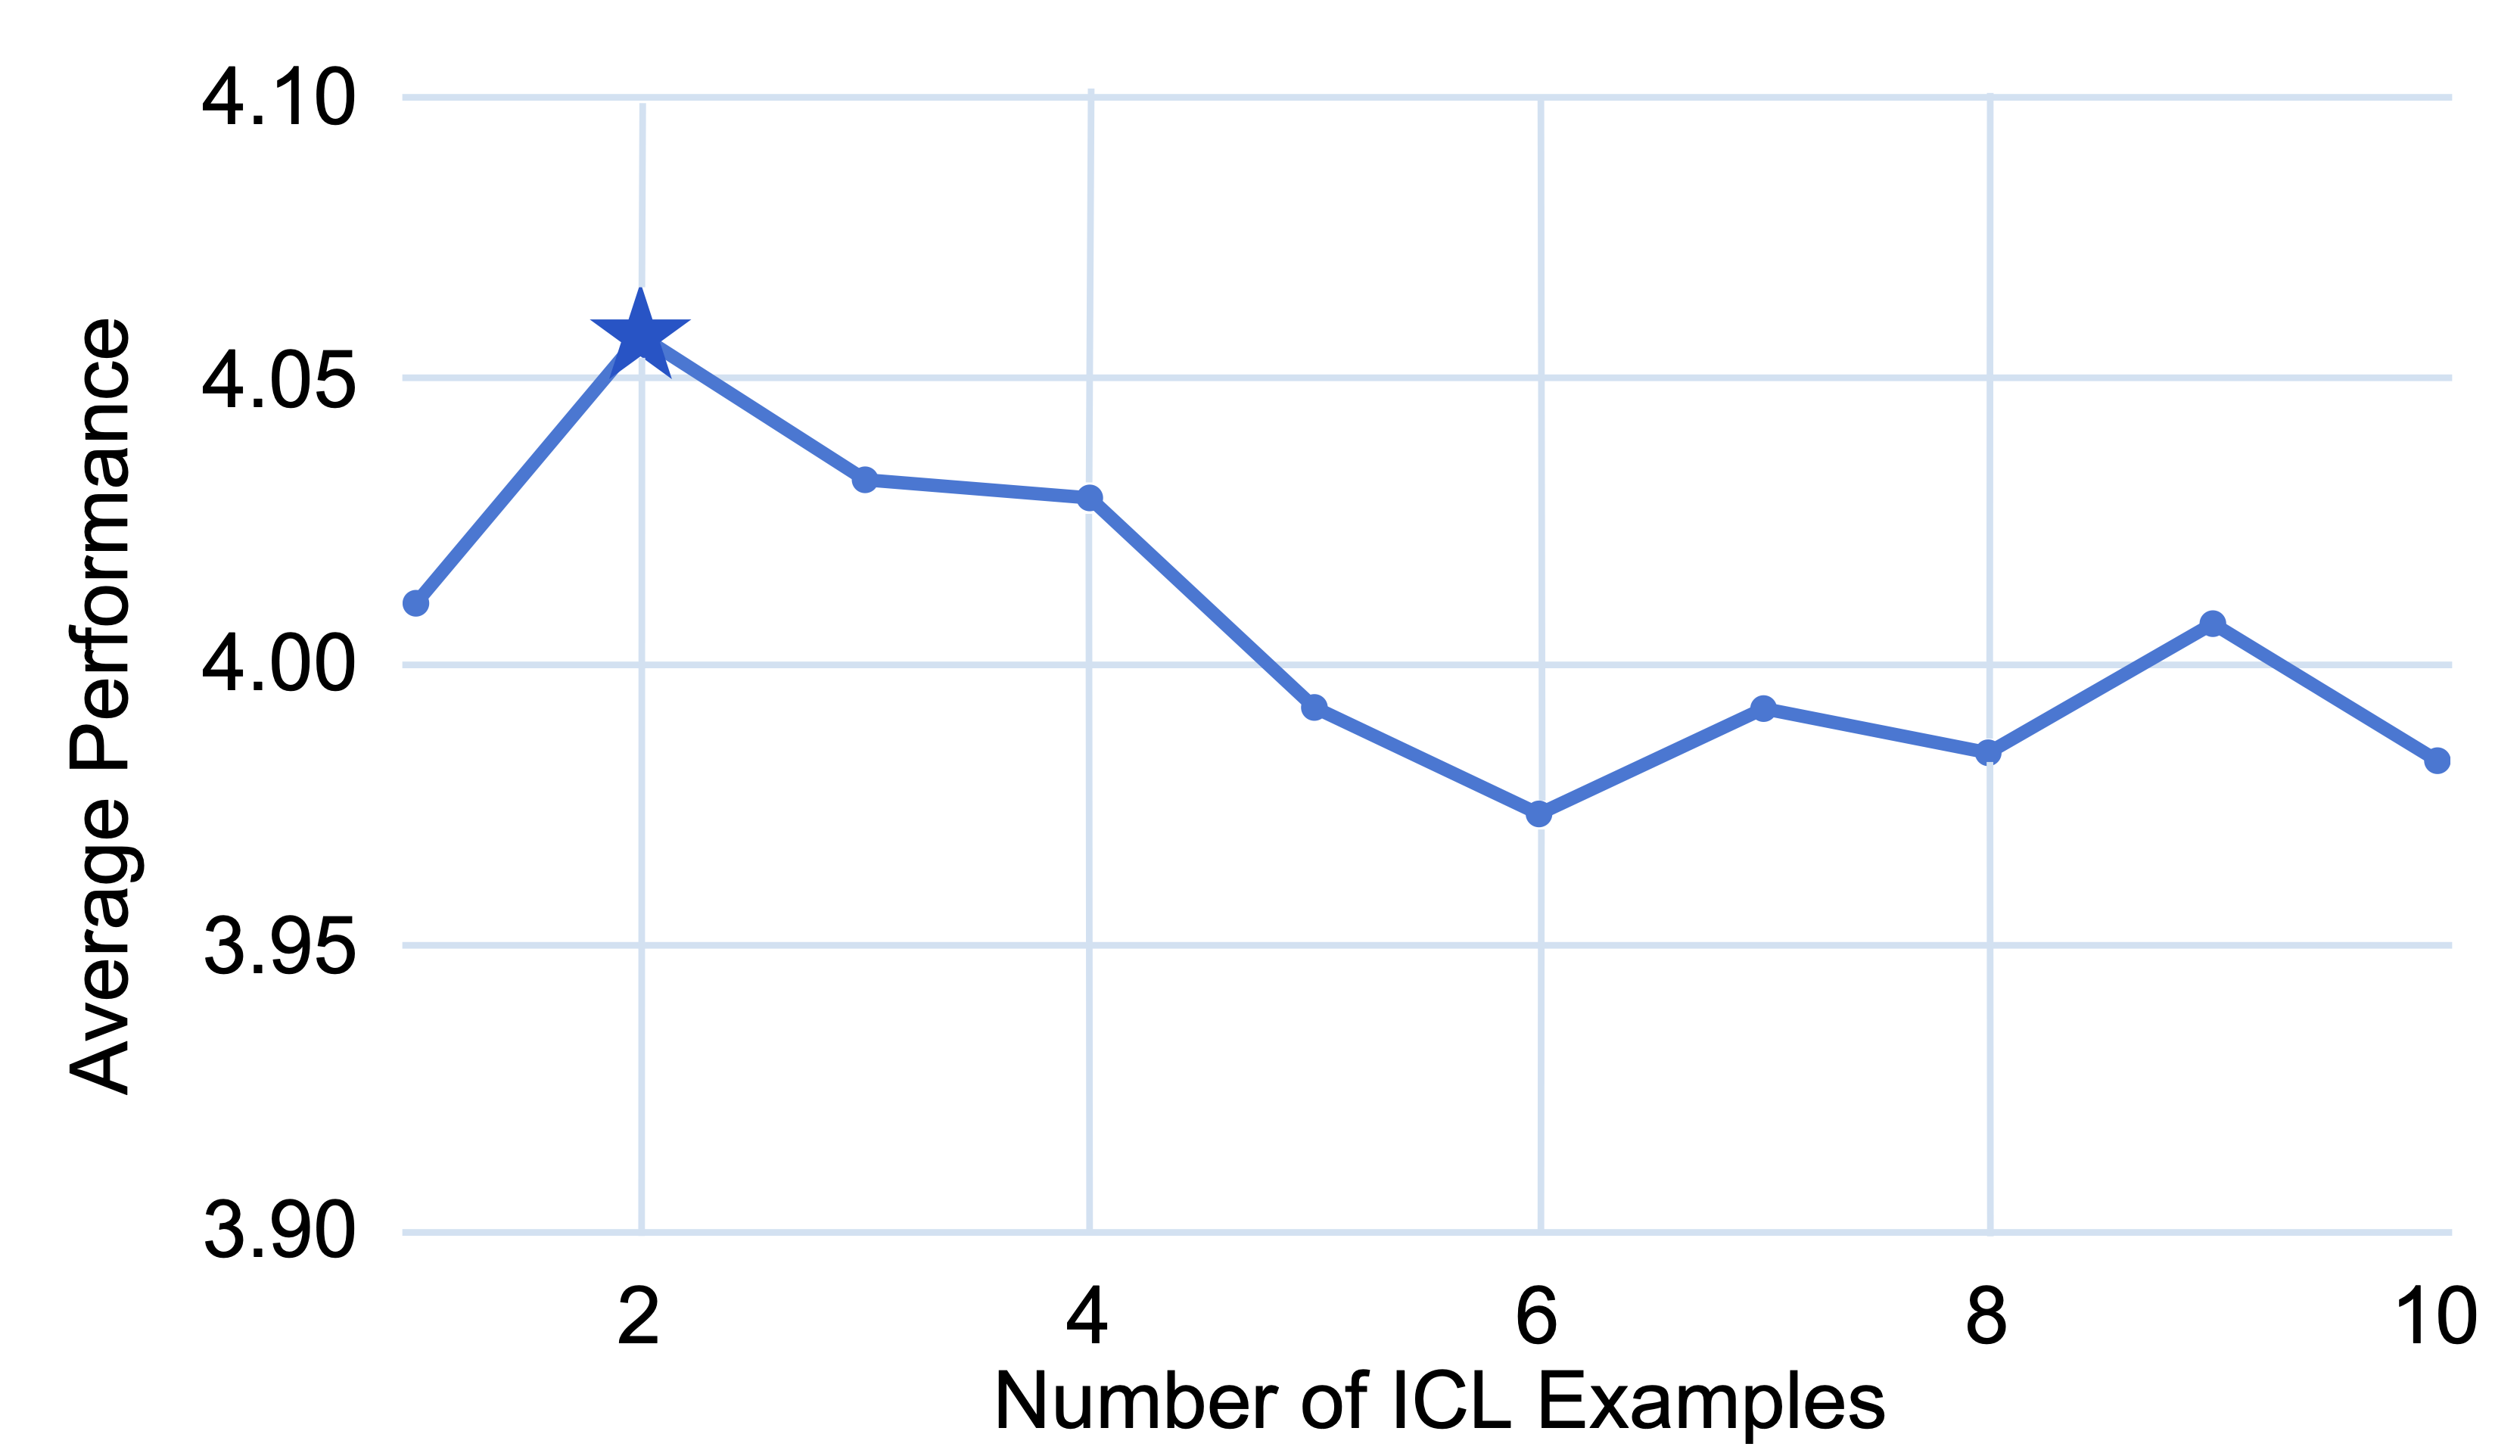
\includegraphics[ width=\linewidth]{images/icl_variation_line_chart_white_bg_v2.png}
    \caption{Performance of Mistral 7b (Instruct)  on varying the number of ICL examples. Two examples give us the best performance with a lower context length cost.}
    \label{fig:icl_variation_chart}
    \vspace{-5pt}
\end{figure}



% Qualitative analysis of gpt prompt

\newcommand{\reduline}[1]{{\color{red}\underline{{\color{black}#1}}}}

\newcommand\dunderline[2][.2pt]{\raisebox{-#1}{\underline{\raisebox{#1}{\smash{\underline{#2}}}}}}

\begin{table}[!t]

\definecolor{Gray}{gray}{0.90}
\newcolumntype{a}{>{\columncolor{Gray}}c}
\centering
\resizebox{1\linewidth}{!}{%
\begin{tabular}{@{}p{10cm}@{}}
\toprule
\textbf{Optimized Alignment Prompt} \\
\midrule
As a helpful and ethical assistant, your primary goal is to provide responses that are accurate, engaging, clear, and emotionally resonant across a wide range of queries. \\
- \ctext[RGB]{230,246,255}{Strive to make complex topics understandable and emotionally engaging, communicating in a human-like and relatable manner. Organize your responses to enhance readability and emotional connection, avoiding overly technical jargon.}  \\
- \ctext[RGB]{233,252,232}{Always acknowledge the limitations of your knowledge, especially when speculating about historical 'what-ifs', future predictions, or interpreting emotions.} \\
- \ctext[RGB]{255,225,255}{Aim for a balance between detailed, informative content and a conversational, engaging tone. Incorporate storytelling elements, examples, analogies, and direct questions to make information relatable.} \\
- \ctext[RGB]{230,246,255}{Avoid overwhelming the user with excessive information; structure your responses to be clear, well-organized, and mindful of the user's cognitive load.}
 \\

 \bottomrule
\end{tabular}%
}
 
\caption{Snippets from the system prompt optimized for \texttt{gpt-3.5-turbo}. The optimized prompt clearly demonstrates improved alignment, addressing potential weaknesses in the model.}
\label{tab:gpt_prompt}
\vspace{-15pt}
\end{table}
\noindent \textbf{Qualitative analysis of optimized prompts}. 
We finally present qualitative results to show \ours' ability to identify a model's alignment weaknesses and tailor system prompts to address them, as shown in Table \ref{tab:gpt_prompt} for \texttt{gpt-3.5-turbo}. The color-coded text in the table highlights specific weaknesses of \texttt{gpt-3.5-turbo} identified by \ours, along with actionable insights. Notably, it highlights \ctext[RGB]{233,252,232}{knowledge limitations of the model}, \ctext[RGB]{255,225,255}{tips to improve engagement} and \ctext[RGB]{230,246,255}{technical verbiage}. For a weaker model like Mistral 7b, \ours identifies the problem of repetitive tokens, which is absent in a strong model like \texttt{gpt-3.5-turbo}. Complete optimized prompts for both models, along with detailed annotations on the differences, can be found in Appendix \ref{sec:prompt_case_study}.  

% radar chart, analyzing various domains/dimensions 

\section{Results}
\label{sec:results}
% 
\begin{table*}[!ht]
    \centering
    \resizebox{\textwidth}{!}{%
    \begin{tabular}{lllllllllcc}
        \toprule             

        Model & $\mathrm{MMMU_{val}}$ &  $\mathrm{MME_{sum}}$ &  $\mathrm{SeedBench_{all}}$ & $\mathrm{OCRBench}$  &  $\mathrm{TextVQA_{val}}$  & $\mathrm{OKVQA}$ & $\mathrm{GQA}$  &  $\mathrm{VizWiz_{val}}$ & $\mathrm{SUM}$  & $\mathrm{Top2}$  \\ 
        
        \hline
\rowcolor{gray!20}
\multicolumn{11}{c}{\textbf{Original Models}} \\
\hline
        Qwen2-VL\footnotesize(base) & 50.11 & 81.44 & 75.85 & \textit{86.00} & \textit{84.12} & 51.43 & 61.80 & 68.32 & 559.07 & 2 \\ 
        LLaVA-OneVision  & 43.44 & 77.04 & 75.44 & 69.60 & 78.47 & 49.57 & 59.84 & 60.97 & 514.37 & 0 \\ 
     % \midrule\
     \hline
       
\rowcolor{gray!20}
\multicolumn{11}{c}{\textbf{Baselines}} \\
\hline

 % \hlinewd{1.5pt}
        Task Arithmetic & 
        48.44\footnotesize(+1.67) & 82.33\footnotesize(+3.09) & 75.81\footnotesize(+0.17) & 77.90\footnotesize(+0.10) & 76.22\footnotesize(-5.08) & 50.60\footnotesize(+0.10) & \textbf{62.26\footnotesize(+1.44)} & 62.76\footnotesize(-1.89) & 536.32\footnotesize(-0.40) &1 
 \\ 
        
        Ties-Merging & \textbf{51.11\footnotesize(+4.34)} & \underline{82.65\footnotesize(+3.41)} & \underline{76.29\footnotesize(+0.64)} & 84.40\footnotesize(+6.60) & 79.56\footnotesize(-1.74) & \underline{52.56\footnotesize(+2.06)} & 61.84\footnotesize(+1.02) & 66.34\footnotesize(+1.69) & 554.75\footnotesize(+18.03) &4 \\ 
        
        DARE-Linear & 43.78\footnotesize(-3.00) & 66.06\footnotesize(-13.18) & 74.32\footnotesize(-1.33) & 72.40\footnotesize(-5.40) & 64.65\footnotesize(-16.65) & 43.41 \footnotesize(-7.09) & 55.13\footnotesize(-5.69) & 50.18\footnotesize(-14.47) & 469.93\footnotesize(-66.79) & 0 \\ 
        
        DARE-Ties & 45.00\footnotesize(-1.78) & 54.43\footnotesize(-24.81) & 74.07\footnotesize(-1.58) & 75.20\footnotesize(-2.60) & 78.54\footnotesize(-2.76) & 49.61\footnotesize(-0.89) & 58.51\footnotesize(-2.31) & 58.05\footnotesize(-6.60) & 493.41 \footnotesize(-43.31) & 0 \\ 
        
        MetaGPT & 50.67\footnotesize(+3.90) & 81.21\footnotesize(+1.97) & \textbf{76.35\footnotesize(+0.70)} & \textbf{85.50\footnotesize(+7.70)} & \underline{83.63\footnotesize(+2.33)} & 52.24\footnotesize(+1.74) & 61.99\footnotesize(+1.17) & \textbf{69.16\footnotesize(+4.51)} & \underline{560.75\footnotesize(+24.03)} & 5  \\[0.5ex] 
        
       \hline
       
\rowcolor{gray!20}
\multicolumn{11}{c}{\textbf{Our Method}} \\
\hline 
                
       
        \ours & 
        \textbf{51.11\footnotesize(+4.34)} & \textbf{83.36\footnotesize(+4.12)} & 76.20\footnotesize(+0.55) & \textbf{85.50\footnotesize(+7.70)} & \underline{83.41\footnotesize(+2.11)} & \textbf{53.56\footnotesize(+3.06)} & \underline{62.02\footnotesize(+1.20)} & \underline{68.40\footnotesize(+3.75)} & \textbf{563.56\footnotesize(+26.84)} & 8 \\ 
        \bottomrule
    \end{tabular}%
        }
    \caption{Results on merging LLaVA-OneVision-7B into Qwen2-VL-7B. All the scores have been scaled to 0-100. SUM refers to the sum of scores on all tasks after scaling. Top2 column represents the number of tasks obtained by this method from the top two among all methods. The number in the parenthesis indicates the performance improvement compared with the average score of original models. The results in the original models that are higher than all model merging methods are highlighted in italics.}
    \label{tab:llava2qwen}
\end{table*}



% 
\begin{table*}[!ht]
    \centering
    \resizebox{\textwidth}{!}{%
    \begin{tabular}{lllllllllcc}
    \toprule
        {Model} & $\mathrm{MMMU_{val}}$ &  $\mathrm{MME_{sum}}$ &  $\mathrm{SeedBench_{all}}$ & $\mathrm{OCRBench}$  &  $\mathrm{TextVQA_{val}}$  & $\mathrm{OKVQA}$ & $\mathrm{GQA}$  &  $\mathrm{VizWiz_{val}}$ & $\mathrm{SUM}$  & $\mathrm{Top2}$  \\ 

\hline
\rowcolor{gray!20}
\multicolumn{11}{c}{\textbf{Original Models}} \\
\hline
        
        CogVLM\footnotesize(base) & 34.80  & 59.23  & 61.22  & \textit{56.50}  & \textit{77.57}  & 60.82  & 59.43  & {37.09}  & {446.66 } &2 \\ 
        LLaVA & 35.10 & 66.68 & 60.52 & 31.30 & 46.04 & 53.42 & \textit{61.94 }& 54.29 & 409.29  &0
 \\
\hline
\rowcolor{gray!20}
\multicolumn{11}{c}{\textbf{Baselines}} \\
\hline
        
        Task Arithmetic & \underline{36.20  \footnotesize(+1.25)} & \underline{65.99}  \footnotesize(+3.03) & \textbf{65.85  \footnotesize(+4.98) }& 51.20  \footnotesize(+7.30) & 68.21  \footnotesize(+6.40) & \textbf{61.92  \footnotesize(+4.80)} & 58.82  \footnotesize(-1.87) & 35.70  \footnotesize(-9.99) & 443.89 
 \footnotesize(+15.91) & 4  \\ 

        
        Ties-Merging & 34.00  \footnotesize(-0.95) & 57.29  \footnotesize(-5.67) & 38.97  \footnotesize(-21.90) & 55.00  \footnotesize(+11.10) & 59.73  \footnotesize(-2.08) & 40.31  \footnotesize(-16.81) & 51.97  \footnotesize(-8.72) & 24.36  \footnotesize(-21.33) & 361.63 
  \footnotesize(-66.35) & 0 \\ 

        
        DARE-Linear & \textbf{36.80  \footnotesize(+1.85)} & 64.08  \footnotesize(+1.12) & \underline{65.07  \footnotesize(+4.20)} & 47.90  \footnotesize(+4.00) & 65.35  \footnotesize(+3.54) & 60.96  \footnotesize(+3.84) & 58.01  \footnotesize(-2.68) & 36.12  \footnotesize(-9.57) & 434.29 
  \footnotesize(+6.31) & 2 \\ 

        
        DARE-Ties & 33.60  \footnotesize(-1.35) & 46.75  \footnotesize(-16.21) & 58.41  \footnotesize(-2.46) & 26.50  \footnotesize(-17.40) & 50.48  \footnotesize(-11.33) & 53.15  \footnotesize(-3.97) & 49.62  \footnotesize(-11.07) & 31.43  \footnotesize(-14.26) & 349.94 
  \footnotesize(-78.04) & 0  \\ 

        
        MetaGPT & 34.70  \footnotesize(-0.25) & 59.37  \footnotesize(-3.59) & 61.29  \footnotesize(+0.42) & \textbf{56.40  \footnotesize(+12.50)} & \textbf{76.96  \footnotesize(+15.15)} & 60.84  \footnotesize(+3.72) & \underline{59.44  \footnotesize(-1.25)} & \underline{36.97  \footnotesize(-8.72)} & \underline{445.97 
 \footnotesize(+17.99)} & 5  \\[0.5ex] 
        
\hline 
\rowcolor{gray!20}
\multicolumn{11}{c}{\textbf{Our Method}} \\
\hline 
      
        AdaMMS & 34.90  \footnotesize(-0.05) & \textbf{69.09  \footnotesize(+6.13)} & 64.12  \footnotesize(+3.25) & \underline{55.70  \footnotesize(+11.80)} & \underline{76.90  \footnotesize(+15.09)} & \underline{61.11  \footnotesize(+3.99)} & \textbf{60.12  \footnotesize(-0.57)} & \textbf{37.27  \footnotesize(-8.42) }& \textbf{459.21  \footnotesize(+31.23)} & 7  \\ 
        
        \bottomrule
    \end{tabular}%
        }
    \caption{Results on merging LLaVA-v1.5-7B into CogVLM-chat-7B.}
     \label{tab:cogvlm}

\end{table*}
% 
\begin{table}[!ht]
    \centering
    % \resizebox{\textwidth}{!}{%
    \begin{tabular}{lccc}
        \toprule
        {Model} & $\mathrm{MMMU_{val}}$ &  $\mathrm{MME_{sum}}$ & $\mathrm{OCRBench}$   \\ 
        \midrule
        \(\alpha\)-1.00 & 50.11  & 81.44  & \textbf{86.00}  \\ 
        \(\alpha\)-0.95 & 49.67  & 81.24  &  85.50 \\ 
        \(\alpha\)-0.90 & 50.56  & 81.46  & 85.50  \\ 
        \(\alpha\)-0.85 & 50.67  & 82.79  & 85.50  \\ 
        \(\alpha\)-0.80 & 51.11  & 82.36  & 85.20  \\ 
        \(\alpha\)-0.75 & 51.11  & 82.88  & 84.60  \\ 
    \(\alpha\)-0.70 & \textbf{51.22}  & 83.36  & 84.40  \\ 
        \(\alpha\)-0.65 & 50.33  & 83.12  & 82.80  \\ 
        \(\alpha\)-0.60 & 50.67  & 83.03  & 80.70  \\ 
        \(\alpha\)-0.55 & 49.33  & \textbf{83.26}  & 79.00  \\ 
        \(\alpha\)-0.50 & 50.00  & 81.37  & 76.40  \\ 
        \(\alpha\)-0.45 & 47.78  & 81.40  & 74.30  \\ 
        \(\alpha\)-0.40 & 47.00  & 82.06  & 71.20 \\
          \midrule
    Oracle\footnotesize(Upper Bound) & 51.22\footnotesize(0.70) & 83.36\footnotesize(0.70) & 85.50\footnotesize(0.10) \\   
       \ours &   51.11\footnotesize(0.80)  & 83.36\footnotesize(0.70)  &  85.50\footnotesize(0.10) \\
     \bottomrule
    \end{tabular}%
    % }
    \caption{Results on0.05 interval. }
    \label{tab:qwen0.05}
\end{table}

\begin{table*}[!ht]
    \centering
    \resizebox{\textwidth}{!}{%
    \begin{tabular}{lllllllllll}
    \toprule
        Method & $\mathrm{MMMU_{val}}$ &  $\mathrm{MME_{sum}}$ &  $\mathrm{SeedBench_{all}}$ & $\mathrm{OCRBench}$  &  $\mathrm{TextVQA_{val}}$ & $\mathrm{ScienceQA}$ & $\mathrm{OKVQA}$ & $\mathrm{GQA}$  &  $\mathrm{VizWiz_{val}}$ & $\mathrm{SUM}$ \\ 
        \midrule

         EM-Full & 51.11 & 83.36 & 76.34 & 85.50  & 83.41 & 85.69 & 53.56 & 62.02 & 68.40  & 563.70   \\ 
         Emb-Full & 50.56 & 83.36 & 76.34 & 85.50  & 83.41 & 85.69 & 53.56 & 61.44 & 68.40  & 562.57   \\ 
         EM-Sample100 & 51.11 & 83.36 & 76.20  & 85.50  & 83.41 & 86.55  & 53.56 & 62.02 & 68.40  & 562.12  \\   
         Emb-Sample100 & 51.11 & 82.36 & 76.34 & 85.50  & 83.41 & 85.69 & 53.56 & 61.44 & 68.40  & 563.56  \\ 
        
        
        \bottomrule
    \end{tabular}%
        }
    \caption{Results on AdaMMS when merging LLaVA-OneVison-7B into Qwen2-VL-7B using exact match (EM-) and sentence embedding (Emb-) to calculate the differences in searching phase, using full test set inputs (-Full) and a sampled subset of 100 inputs (-Sample100).}
     \label{tab:embedding}

\end{table*}

\begin{table}[ht]
    \centering
    % \resizebox{\textwidth}{!}{%
    \begin{tabular}{lccc}
        \toprule
        {Model} & $\mathrm{MMMU_{val}}$ &  $\mathrm{MME_{sum}}$ & $\mathrm{OCRBench}$   \\ 
        \midrule
        \(\alpha\)-0.00 & 50.11  & 81.44  & \textbf{86.00}  \\ 
       
        \(\alpha\)-0.10 & 50.56  & 81.46  & 85.50  \\ 
        
        \(\alpha\)-0.20 & 51.11  & 82.36  & 85.20  \\ 
       
    \(\alpha\)-0.30 & \textbf{51.22}  & \textbf{83.36}  & 84.40  \\ 
     
        \(\alpha\)-0.40 & 50.67  & 83.03  & 80.70  \\ 
     
        \(\alpha\)-0.50 & 50.00  & 81.37  & 76.40  \\ 
     
        \(\alpha\)-0.60 & 47.00  & 82.06  & 71.20 \\
          \midrule
    Oracle & 51.22\footnotesize(0.30) & 83.36\footnotesize(0.30) & 85.50\footnotesize(0.10) \\   
       \ours &   51.11\footnotesize(0.20)  & 83.36\footnotesize(0.30)  &  85.50\footnotesize(0.10) \\
     \bottomrule
    \end{tabular}%
    % }
    \caption{Results with $\alpha$ granularity of 0.1 when merging LLaVA-OneVision-7B into Qwen2-VL-7B. The values in parentheses indicate the selected $\alpha$. Oracle represents the best possible performance (upper bound) for each task, while AdaMMS shows the results achieved by our unsupervised selection method.}
    \label{tab:qwen0.1}
\end{table}


\begin{table}[!ht]
    \centering
     \resizebox{0.4 \textwidth}{!}{%
    \begin{tabular}{lcc}
    \\
    \hline
  % Model & \multicolumn{2}{c}{OCRBench} &
   
        \rowcolor{gray!20}
\multicolumn{3}{c}{\textbf{Original Models}} \\
\hline 

        LLaVA-OneVision & 69.60  & 69.60  \\ 
        Qwen2-VL & 86.00  & 86.00  \\ 

          \hline

        Merging-Base & LLaVA-OneVision & Qwen2-VL \\ 
        
         \hline       
        \rowcolor{gray!20}
        
\multicolumn{3}{c}{\textbf{Baselines}} \\
\hline 
        Task Arithmetic  & 68.10  & 77.90  \\ 
        Ties-Merging  & 56.10  & 84.40  \\ 
        DARE-Linear  & 63.90  & 72.40  \\ 
        DARE-Ties  & 64.40  & 75.20  \\ 
        MetaGPT & 38.40  & \textbf{85.50}  \\ 
         \hline       
        \rowcolor{gray!20}
\multicolumn{3}{c}{\textbf{Linear Interpolation}} \\
\hline 
        $\alpha$-0.10 & 70.60  & 85.50  \\ 
        $\alpha$-0.20 & 71.70  & 85.20  \\ 
        $\alpha$-0.30 & 69.90  & 84.40  \\ 
        $\alpha$-0.40 & 67.00  & 80.70  \\ 
        $\alpha$-0.50 & 62.00  & 76.40  \\ 
        $\alpha$-0.60 & 54.40  & 71.30  \\ 
 \hline       
        \rowcolor{gray!20}
\multicolumn{3}{c}{\textbf{Our Method}} \\
\hline 
              
        AdaMMS & \textbf{70.60}  & \textbf{85.50} \\ \hline
    \end{tabular}
    }
    
    \caption{Results on OCRBench when merging LLaVA-OneVision-7B and Qwen2-VL-7B. }
    \label{tab:reverse}
\end{table}

As described in Section~\ref{models}, the main results on distinct vision-language benchmarks are conducted with two representative MLLM pairs. Specifically, Table~\ref{tab:llava2qwen} shows the results of merging LLaVA-OneVision-7B's parameters into Qwen2-VL-7B's parameters and architecture, and Table~\ref{tab:cogvlm} shows the results of merging LLaVA-v1.5-7B's parameters into CogVLM-chat-7B's parameters and architecture. Results of other model pairs and larger models can be found in Appendix~\ref{appendix:additional}.

\textbf{\ours  addresses the challenges of merging for heterogeneous MLLMs and outperforms strong baselines.} As demonstrated in Table~\ref{tab:llava2qwen} and Table~\ref{tab:cogvlm}, our proposed \ours model merging method achieves the highest cumulative performance scores across both MLLM pairs, indicating its effectiveness in merging heterogeneous MLLMs. Ranks among the top two performs in 8 out of 9 metrics in Table~\ref{tab:llava2qwen} and 7 metrics in Table~\ref{tab:cogvlm}, demonstrating its consistent ability to adaptively improve performance across most tasks. 
Moreover, our method stands out as the only approach where the merged model significantly outperforms both pre-merged models, achieving an average gain of +3.36~(total gain of +26.84) over Qwen2-VL and +3.90 over CogVLM across 8 tasks.
Given that most baseline methods employ supervised search techniques that incorporate additional information, our unsupervised search approach demonstrates exceptional performance on vision-language benchmarks, as detailed illustrated in Appendix~\ref{appendix:unsupervised}. 
%结合数字,列出来特殊性,有信息量的。
%比较两个表

\textbf{The proposed unsupervised hyper-parameter selection method is able to select a near-optimal $\alpha$.} We evaluate the performance across different coefficient values $\alpha$, comparing the results obtained through our unsupervised hyper-parameter selection method against those achieved with the optimal $\alpha$ chosen by the actual best results, which serves as the theoretical upper bound. As shown in Table \ref{tab:qwen0.1}, our method consistently performs remarkably close to this upper bound, with a maximum deviation of only 0.5 points. These results demonstrate the capability of our method to accurately identify near-optimal $\alpha$ values, achieving performance levels approaching the theoretical best.

% As shown in Table \ref{tab:qwen0.1}, we compare the performance of $\alpha$ chosen by our unsupervised hyper-parameter selection method, and the performance of the optimal $alpha$ chosen by the Oracle, serving as the upper bound of our method. In these benchmarks, our method is at most 0.5 points below the upper bound. The results indicates that our method can accurately select the near-optimal $\alpha$, obtaining performances close to the best possible choice. 

Note that on the OCRBench and TextVQA benchmarks, all model merging methods, including \ours, show a performance drop compared to the original base model.
We hypothesize that this is due to the large performance gap between the two original models on these benchmarks.
Even though, \ours still outperforms most of the baselines, showing the robustness of our method on various scenarios.

% : while original models with similar performance tends to benefit from model merging, merging a worse model to the base model on certain tasks may lead to performance drop. 
% TODO: 这段也有点分析,先不写上

% 
\begin{table}[!ht]
    \centering
    \begin{tabular}{llll}
     \toprule
        \textbf{Model} & $\mathrm{MMMU_{val}}$ &  $\mathrm{MME_{sum}}$ & $\mathrm{OCRBench}$   \\ 
        \midrule
       
        alpha-0.00 & 50.11  & 81.44  & \textbf{86.00}  \\ 
        alpha-0.02 & 49.67 & 81.69  & \textbf{86.00}  \\ 
        alpha-0.04 & 50.00  & 80.96  & 85.50  \\ 
        alpha-0.06 & 49.89  & 81.13  & 85.30  \\ 
        alpha-0.08 & 49.33  & 81.32  & 85.50  \\ 
        alpha-0.10 & 50.56  & 81.46  & 85.50  \\ 
        alpha-0.12 & 50.11  & 81.92  & 85.70  \\ 
        alpha-0.14 & 50.78  & 82.39  & 85.70  \\ 
        alpha-0.16 & 50.44  & 82.05  & 85.70  \\ 
        alpha-0.18 & 51.00  & 83.02  & 85.40  \\ 
        alpha-0.20 & 51.11  & 82.36  & 85.20  \\ 
        alpha-0.22 & 50.11  & 83.37  & 85.30  \\ 
        alpha-0.24 & 51.11  & 82.72  & 85.00  \\ 
        alpha-0.26 & 51.11  & 82.80  & 84.70  \\ 
        alpha-0.28 & 51.11  & \textbf{83.63}  & 84.40  \\ 
        alpha-0.30 & \textbf{51.22}  & 83.36  & 84.40  \\ 
        alpha-0.32 & 51.00  & 83.47  & 83.90  \\ 
        alpha-0.34 & 50.33  & 83.48  & 83.10  \\ 
        alpha-0.36 & 50.22  & 83.22  & 82.10  \\ 
        alpha-0.38 & 50.00  & 82.96  & 81.30  \\ 
        alpha-0.40 & 50.67  & 83.03  & 80.70  \\ 
        alpha-0.42 & 50.11  & 83.37  & 79.80  \\ 
        alpha-0.44 & 49.89  & 83.02  & 78.90  \\ 
        alpha-0.46 & 49.78  & 83.13  & 78.20  \\ 
        alpha-0.48 & 48.89  & 82.57  & 77.30  \\ 
        alpha-0.50 & 50.00  & 81.37  & 76.40 \\ 
          \midrule
        diff3-EM  & 50.44 & 83.42 &85.30 \\
         \bottomrule
    \end{tabular}%
    % }
    \caption{Results on 0.02 interval. }
    \label{tab:qwen0.02}
\end{table}
%好像有点不连贯。 先说总体每个任务都不错,为什么。 然后baseline中metagpt表现还可以,因为他选了综合最优的alpha。然后是qwen达到了最优的效果,证明方法的优越性。最后是limit证明可口扩展性。
% Our primary objective is to adaptively integrate two MLLMs into a single MLLM with better performance on given tasks without labeled data. Unlike all baseline methods, which are task-agnostic and may underperform in scenarios with substantial discrepancies between candidate MLLMs, our approach tailors a specific MLLM to each task. Despite this customization, the additional costs are minimal and also save storage. Mms-merging requires only 100 unlabeled samples for the search phase, and we store only the hyperparameter coefficient, rather than the entire model. 

% Overall, our mms-merging consistently achieved optimal performance across all evaluated tasks. Metagpt \cite{metagpt} performed suboptimal and stable, which computed the ideal coefficient value for linear interpolation through analytical reasoning but ignored difference among tasks. Other baselines were unable to search for the optimal hyperparameter value due to the absence of label data, so we assigned empirical values for them.


%  As shown in Table \ref{tab:llava2qwen}, when Llava-one-vision-Qwen \cite{llava-onevison} was merged with Qwen(base) \cite{qwen2-vl}, our mms-merging achieved State-of-the-Art performance in 7B MLLMs on certain tasks and demonstrated the strongest overall capabilities. This proves our effectiveness and potentiality.
 
%  The final row displays the results obtained from sampling only 100 samples (10\%-0.5\% of original datasets). It is evident that the performance remains consistent with the full dataset.
 
%  % Our results revealed that for the OCRBench and TextVQA datasets, none of the merging methods outperformed the original MLLM. This trend was also observed in most other model fusions, leading us to suppose that the original models may have already overfitted to these two popular datasets.

  
% Overall, our approach outperform the baseline and original MLLM. Besides, our method exhibits considerable robustness, stability and scalability. 





\section{Analysis}
\label{sec:ana}
\begin{figure}
    \centering
    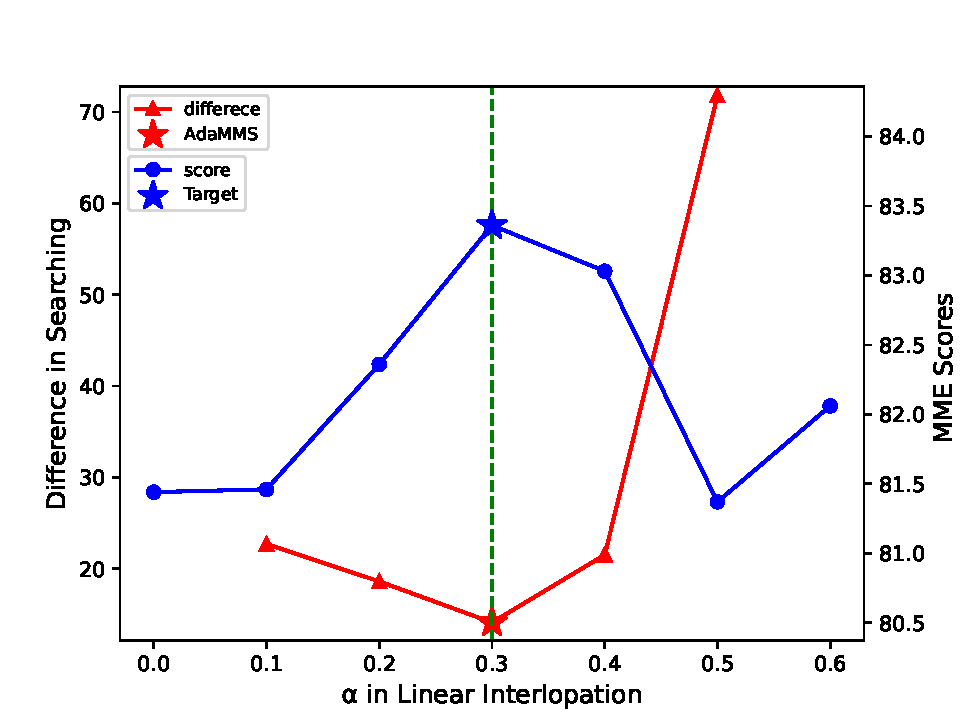
\includegraphics[width=0.4 \textwidth, bb=0 0 461 346]{figure/diff_acc_plot_new.pdf}
    \caption{Results on merging LLaVA-v1.5-7B into Qwen2-VL-7B. The $\alpha$ with the best perfo, bb=0 0 461 346rmance are the same as the $\alpha$ with the fewest response differences.}
    \label{fig:difference}
\end{figure}

%同构模型融合,以及searching方法的有效性。
\subsection{Different Factors for Calculating Generation Consistency}
We conducted analytical experiments on our generation consistency calculation methods, focusing on two key factors: the choice between using a 100-sample subset versus the complete dataset, and the selection of evaluation metrics. In the searching step of our method, we employed an exact match metric to calculate $\operatorname*{DiffCnt}$ in Algorithm~\ref{alg:composition}, which serves as our generation consistency indicator for model performance prediction. Given that exact match is a binary, rigorous evaluation metric, we explored an alternative, more flexible approach to measure generation consistency. Specifically, we computed the cosine similarity between sentence embeddings generated by all-MiniLM-L6-v2 \cite{sentence-bert}, which was used to calculate $\operatorname*{DiffCnt}$. The analysis results are presented in Table~\ref{tab:embedding}. Although embeddings theoretically offer more fine-grained semantic representations, our results demonstrate that the embedding-based metric performs comparably to the exact match metric. Furthermore, our experiments confirm that sampling 100 instances achieves results nearly equivalent to the complete dataset.


% In the searching step of \ours, we employed exact match metric to calculate $\operatorname*{DiffCnt}$ in Algorithm~\ref{alg:composition}, which is the the indicator of generation consistency that is used to predict the model performance.
% Since exact match is a binary, hard-judgment metric, we investigate an alternative, softer metric to capture generation consistency. Specifically, we compute the cosine similarity between sentence embeddings generated by all-MiniLM-L6-v2 \cite{sentence-bert}, which we use to calculate $\operatorname*{DiffCnt}$.
% % Given that the model often produces responses in sentence format, we incorporated embedding method to assess the consistency of responses, aiming to compare the effectiveness of these two evaluation approaches. 
% While embeddings theoretically offer a fine-grained semantic representation, the results depicted in Table \ref{tab:embedding} reveal that the embedding metric performs similarly with the exact match metric.
% % This disparity can be attributed to the fact that the consistency evaluated by the embedding metric does not correspond to alterations in the models' hidden states.
% % The initial assumption was that the responses from both models would identical, indicating similarity in their hidden states and loss, thereby illustrating a smoother model within the vicinity of that alpha value in the linear interpolation space.
% This indicates that our choice in the main experiments of the exact match metric is sufficient for demonstrating the generation consistency for performance estimation.


\subsection{Merging with Large Performance Gap}

As discussed in Section~\ref{sec:results}, all model merging methods experience performance drop after the merging on two benchmarks, OCRBench and TextVQA. It shows that merging a model with significant \textit{lower} performance into the base model will decrease the performance on the task. Conversely, in Table~\ref{tab:reverse}, the merging from Qwen2-VL-7B to LLaVA-OneVision-7B shows that merging a model with significant \textit{higher} performance into the base model will not necessarily improve the model performance. And in this case, \ours is the only model merging method that resists the performance drop after merging.
In general, we observed that original models with similar performance tends to benefit from model merging, while original models with large performance gap do not.

\begin{figure}
    \centering
    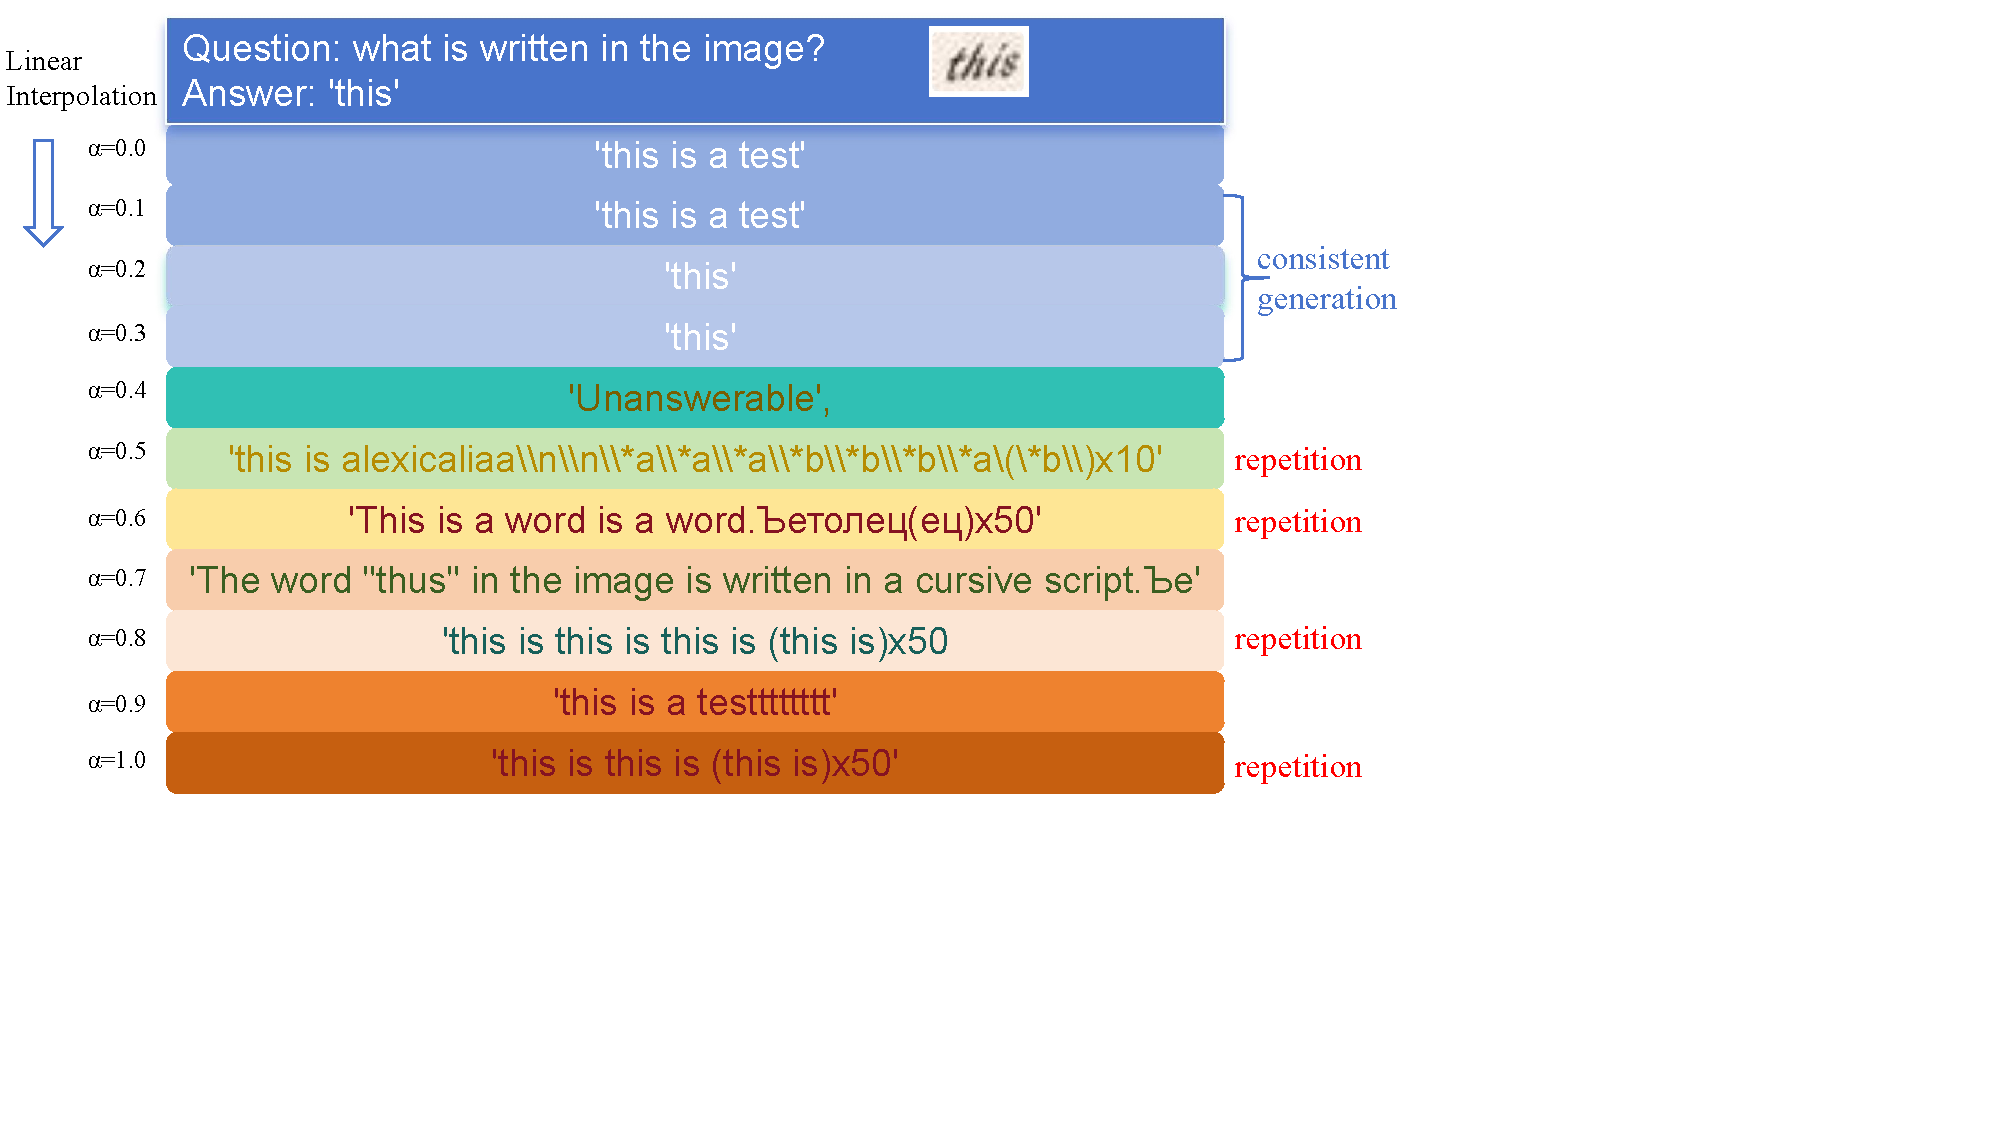
\includegraphics[width=\linewidth, bb=0 0 678 389]{figure/crop_diff-case.pdf}
    \caption{Model responses with the change of $\alpha$ in linear interpolation. Similar colors indicate similar responses.  }
    \label{fig:asymmetry}
\end{figure}

% The training data for different MLLMs varies, leading to performance differences across tasks. Model performance tends to be more stable when merging on tasks with smaller differences. Conversely, merging on tasks with large gap tends to unstable performance. Our mms-merging method exhibits strong stability, preventing models with poor performance from dragging down the overall results. As shown in Table \ref{tab:llava2qwen}  there is a 17\% gap between the two models for OCRBench \cite{ocrbench}. Only our mms-merging and MetaGPT \cite{metagpt} methods maintain the high performance of Qwen2\_VL \cite{Qwen2-VL-7B}.
%不同的MLLM训练数据不一样,这就导致了他们在任务上的表现有差异。在差异小的任务上进行融合时模型表现会比较稳定。而在差异大的任务进行融合则会表现动荡。 我们的方法具有很好的稳定性,可以避免表现差的模型拉低结果。可以看到表1中的OCRBENCH,两个模型相差17%,只有我们的mms-merging和metagpt保持住qwen2的好表现。
\subsection{Asymmetry in the Parameter Space of Heterogeneous Models} \label{sec:asymmetry_sec}
In Section~\ref{impl}, we discussed that merging with large $\alpha$ often results in collapsing language ability. To validate our choice of the subinterval $[0, 0.6]$ in determining candidates of $\alpha$, we demonstrate this phenomenon in Figure~\ref{fig:asymmetry}, which shows that the model generates consistently near the parameters of the base model with small $\alpha$, and collapses gradually with larger $\alpha$. We attribute the phenomenon to the asymmetry in the parameter space, as the two original models have unequal status that comes from the choice of base architecture.

\subsection{Selection of Granularity for \texorpdfstring{$\alpha$}{alpha}}
\label{sec:interval}
To validate our choice of the granularity in Section~\ref{impl}, we conducted additional experiments with various granularities of $\alpha$ candidates on n MME and OCRBench when merging LLaVA-OneVison-7B into Qwen2-VL-7B. As shown in Appendix~\ref{appendix:granularity}, the result shows that the difference of selected $\alpha$ and model performance do not change significantly with different granularities. This shows that our choice of granularity as 0.1 would result in comparable performance, with less computation cost.

% Generally speaking, there is a trade-off between the granularity of $\alpha$ and the results. The finer grained the alpha, the better the potential outcomes, but the higher the cost. In practice, we found that refining the granularity of $\alpha$  to 0.05 or 0.02 did not result in significant improvements. They are displayed in the Figure \ref{sec:interval}. Therefore selecting an interval of 0.1 for alpha in the main experiment was sufficient.





% \subsection{Homogeneous V.S. Heterogeneous Merging}
% % 我们的diff方法在同构模型中仍然有效。需要强调的是同构模型融合的所有结果增益都比较小,不如异构融合带来的增益。
% Both ShareGPT4V and LLaVA-1.5 include three integral components:(1)A vision encoder utilizing the CLIP-Large model.(2) A projector, two layer multi-layer perception (MLP),  to connect the vision and language modalities. (3) A LLM derived from LLaMA2.

% The merging method applied to these two homogeneous MLLMs is identical to that used on homogeneous LLMs. The results after merging remain stable, but the improvements are minimal. Therefore, we argue that the gains of merging heterogeneous MLLMs surpass homogeneous ones.
% 
\begin{table*}[!ht]
    \centering
    \resizebox{\textwidth}{!}{%
    \begin{tabular}{llllllllll}
    \toprule
     \textbf{Model} & $\mathrm{MMMU_{val}}$ &  $\mathrm{MME_{sum}}$ &  $\mathrm{SeedBench_{all}}$ & $\mathrm{OCRBench}$  &  $\mathrm{TextVQA_{val}}$  & $\mathrm{OKVQA}$ & $\mathrm{GQA}$  &  $\mathrm{VizWiz_{val}}$ & $\mathrm{SUM}$ \\ 
        \midrule
     0.0(Sharegpt) & 36.60  & 65.32  & 63.72  & 37.60  & 46.88  & 50.98  & 63.27  & 60.38  & 424.75  \\ 
        0.1 & 36.20  & 65.94  & 63.77  & 37.70  & 47.11  & 52.31  & 63.35  & 60.30  & 426.68  \\ 
        0.2 & 36.90  & 66.32  & 63.73  & 37.40  & 47.28  & 53.78  & 63.40  & 60.55  & 429.36  \\ 
        0.3 & 35.80  & 67.13  & 63.42  & 37.30  & 47.42  & 54.14  & 63.44  & 60.42  & 429.07  \\ 
        0.4 & 36.20  & 67.20  & 63.29  & 37.20  & 47.60  & 54.51  & 63.29  & 59.85  & 429.14  \\ 
        0.5 & 36.40  & 67.63  & 63.39  & 37.20  & 47.58  & 54.60  & 63.13  & 59.37  & 429.30  \\ 
        0.6 & 37.10  & 67.20  & 63.22  & 36.80  & 47.28  & 54.65  & 62.95  & 59.18  & 428.38  \\ 
        0.7 & 37.00  & 66.51  & 63.10  & 36.70  & 46.93  & 54.67  & 62.77  & 58.64  & 426.32  \\ 
        0.8 & 36.30  & 66.24  & 62.95  & 36.50  & 46.78  & 54.53  & 62.70  & 58.10  & 424.10  \\ 
        0.9 & 36.30  & 66.48  & 62.72  & 35.60  & 46.44  & 53.82  & 62.57  & 57.41  & 421.34  \\ 
        1.0(LLaVA) & 34.90  & 67.42  & 62.20  & 34.60  & 46.04  & 53.05  & 62.32  & 56.81  & 417.34  \\ 
        Task Arithmetic  & 36.10  & 69.61  & 63.40  & 37.00  & 50.65  & 53.37  & 63.13  & 59.29  & 432.55  \\ 
        Ties-Merging  & 35.90  & 69.57  & 61.73  & 35.70  & 50.36  & 54.44  & 63.17  & 54.89  & 425.76  \\ 
        DARE-Linear  & 36.30  & 69.40  & 63.36  & 37.40  & 50.70  & 53.71  & 63.06  & 59.55  & 433.48  \\ 
        DARE-Ties  & 32.80  & 58.59  & 56.49  & 32.60  & 44.11  & 50.20  & 57.23  & 43.78  & 375.80  \\ 
        MetaGPT & 36.30  & 70.58  & 63.44  & 37.10  & 50.93  & 53.57  & 63.23  & 59.72  & 434.87  \\ 
        diff3-sample0.1-EM & 36.30  & 66.48  & 63.77  & 37.30  & 47.60  & 54.14  & 63.13  & 60.55  & 429.27 \\ 
        \bottomrule
    \end{tabular}%
        }
    \caption{Results on various benchmark when merging LLaVA-v1.5-7B into ShareGPT-4V-7B.}
     \label{tab:llava2share}

\end{table*}



% \begin{figure}
%   \centering 
%  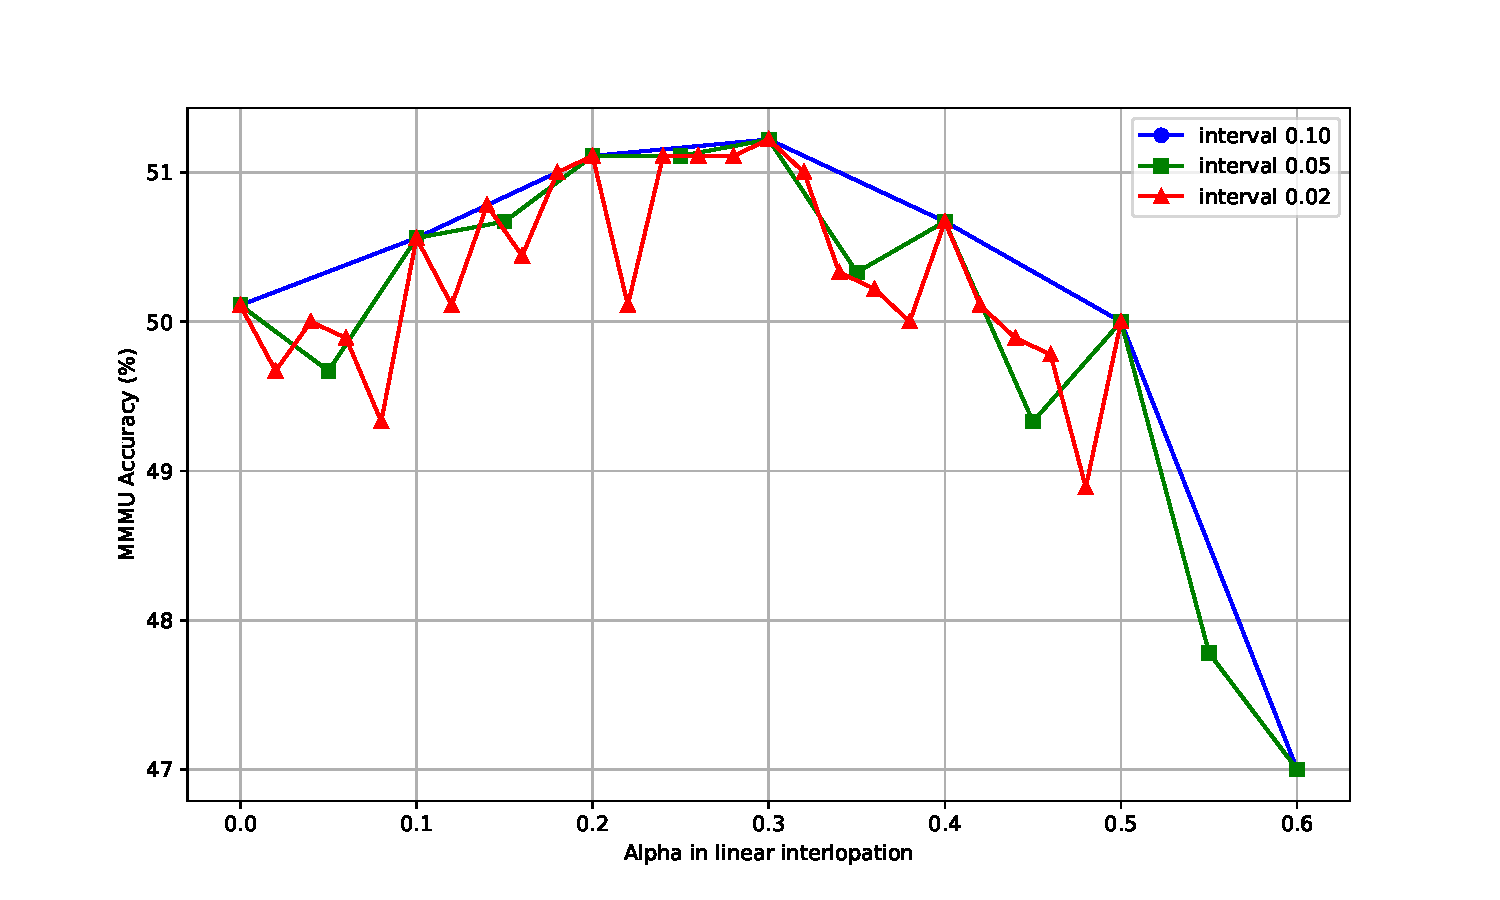
\includegraphics[width=0.4\textwidth]{figure/mmmu_mme_ocr.pdf}
%   \caption{Results with alpha intervals of 0.1, 0.05, and 0.02 in linear interpolation.}
%   \label{intervals}
% \end{figure}



 % 
\begin{table*}[!ht]
    \centering
    \resizebox{\textwidth}{!}{%
    \begin{tabular}{lclllllllllc}
        \toprule             

        Model & $\mathrm{Unsupervised}$ & $\mathrm{MMMU_{val}}$ &  $\mathrm{MME_{sum}}$ &  $\mathrm{SeedBench_{all}}$ & $\mathrm{OCRBench}$  &  $\mathrm{TextVQA_{val}}$  & $\mathrm{OKVQA}$ & $\mathrm{GQA}$  &  $\mathrm{VizWiz_{val}}$ & $\mathrm{SUM}$  & $\mathrm{Top2}$  \\ 
        \hline

\rowcolor{gray!20}
\multicolumn{12}{c}{\textbf{Original Models}} \\
\hline
 mPLUG-Owl2\footnotesize(base) & ~ & 34.90  & 62.80  & 59.41  & 34.10  & 55.13  & 60.98  & 56.11  & 32.07  & 395.50  \\ 
     CogVLM & ~  & 34.80  & 59.23  & 61.22  & \textit{56.50}  & \textit{77.57}  & 60.82  & \textit{59.43}  & \textit{37.09}  & \textit{446.66} \\ 
       
    
     \hline
       
\rowcolor{gray!20}
\multicolumn{12}{c}{\textbf{Baselines}} \\
\hline
Task Arithmetic &$\times$ & \underline{38.80\footnotesize(+3.95)} & \textbf{64.65\footnotesize(+3.63)} & \textbf{60.85\footnotesize(+0.53)} & \textbf{31.50\footnotesize(-13.80)} & \textbf{56.99\footnotesize(-9.36)} & 60.93\footnotesize(+0.03) & \underline{54.44\footnotesize(-3.33)} & \textbf{32.76\footnotesize(-1.82)} & \textbf{400.92\footnotesize(-20.16)} & 8 \\

        Ties-Merging &$\times$ & 27.9\footnotesize(-6.95) & 48.96\footnotesize(-12.06) & 52.32\footnotesize(-8.00) & 24.30\footnotesize(-21.00) & 42.10\footnotesize(-24.25) & 54.15\footnotesize(-6.75) & 43.02\footnotesize(-14.75) & 27.56\footnotesize(-7.02) & 320.31\footnotesize(-100.77) &0 \\ 
        
        DARE-Linear & $\times$ &37.60\footnotesize(+2.75) & 62.44\footnotesize(+1.42) & 59.81\footnotesize(-0.51) & 30.90\footnotesize(-14.40) & 56.41\footnotesize(-9.94) & \underline{61.07\footnotesize(+0.17)} & 54.11\footnotesize(-3.66) & 32.42\footnotesize(-2.16) & 394.76\footnotesize(-26.32) & 1\\ 
        
        DARE-Ties & $\times$ &32.00\footnotesize(-2.85) & 57.90\footnotesize(-3.12) & 57.62\footnotesize(-2.70) & 24.10\footnotesize(-21.20) & 43.84\footnotesize(-22.51) & 51.56\footnotesize(-9.34) & 52.04\footnotesize(-5.73) & 25.67\footnotesize(-8.91) & 344.73\footnotesize(-76.35) & 0\\
        
        MetaGPT & $\checkmark$&31.30\footnotesize(-3.55) & 56.81\footnotesize(-4.21) & 50.81\footnotesize(-9.51) & 29.30\footnotesize(-16.00) & 37.96\footnotesize(-28.39) & 43.02\footnotesize(-17.88) & 34.12\footnotesize(-23.65) & 15.84\footnotesize(-18.74) & 299.16\footnotesize(-121.92)  &0
          \\[0.5ex] 
               \hline       
\rowcolor{gray!20}
\multicolumn{12}{c}{\textbf{Our Method}} \\
\hline                    
       AdaMMS &$\checkmark$& \textbf{39.10\footnotesize(+4.25)} & \textbf{64.65\footnotesize(+3.63)} & \underline{60.16\footnotesize(-0.16)} & \underline{30.60\footnotesize(-14.70)} & \underline{55.88\footnotesize(-10.47)} & \textbf{62.11\footnotesize(+1.21)} & \textbf{55.61\footnotesize(-2.16)} & \underline{32.69\footnotesize(-1.89)} & \underline{400.80\footnotesize(-20.28)} & 9\\
        \bottomrule
    \end{tabular}%
        }
    \caption{Results on merging CogVLM-7B into mPLUG-Owl2-7B.}
    \label{tab:cog2mplug}
\end{table*}



% \input{floats/llava2mplug}
\section{Conclusion}
\label{sec:conclusion}

In this work, we propose a novel model merging method \ours to address the challenges in merging heterogeneous MLLMs. We first connect the parameters of different MLLMs through a mapping function, enabling merging operations. We then apply linear interpolation to the mapped model weights to adaptively optimize performance across tasks. To optimize the interpolation coefficient without labeled data, we introduce an unsupervised hyperparameter searching method based on our discovery in the parameter space: model performance can be estimated through the generation consistency. We demonstrate that 100 data samples are enough to search for near-optimal coefficients effectively.
Extensive experimental results show that \ours outperforms existing model merging methods for MLLMs and successfully addresses the challenges in merging heterogeneous MLLMs. We hope that our work mitigates the limitations of heterogeneous model merging methods and provides valuable insights for future research on unsupervised performance estimation and optimization.
% in parameter space through our hyperparameter selection method.

% tackle the challenges in model merging for heterogeneous MLLMs by proposing a novel model merging method named \ours. In \ours, MLLMs with different language model architectures are first connected with a mapping function, allowing merging operations to be applied. Then we apply linear interpolation on the mapped model weights to adaptively optimize the performance on each task. To search for the linear interpolation coefficient without the need of labeled data, we proposed a unsupervised hyper-parameter selection method, which is based on our discovery on the parameter space that the model performance can be estimated through the consistency of generated responses. We demonstrated that it only needs a small amount of responses to search for the near-optimal coefficient in an efficient way. Extensive results shows that \ours outperforms previous model merging methods on MLLMs, tackles the challenges in merging heterogeneous MLLMs. We hope our work can unlock the constraints on model merging methods for heterogeneous models, and provide insights to future research on unsupervised performance estimation on parameter space through our hyper-parameter selection method.

\section*{Acknowledgment}
    
This work is supported by the National Key R\&D Program of China (2022ZD0160502) and the National Natural Science Foundation of China (No. 62276152).

{
    \small
    \bibliographystyle{ieeenat_fullname}
    \bibliography{main}
}

% WARNING: do not forget to delete the supplementary pages from your submission 
\clearpage
\appendix
\setcounter{page}{1}
\maketitlesupplementary

\section{Implementation Details}
We follow prior studies\cite{coop, cocoop, prograd, kgcoop, maple, tcp, mma} and adopt a 16-shot learning setting across all experiments, except for the few-shot learning tasks. The ViT-B/16\cite{vit} variant of the CLIP model serves as the visual backbone for all experimental setups. Hand-crafted text prompts from prior methods\cite{clip, coop, tip-adapter} are utilized and described in detail in \cref{datasets}. Optimization is performed using the AdamW optimizer with an initial learning rate of 0.001. All our models are trained with mix-precision for speeding up. For the larger ImageNet dataset, we employ a batch size of 32, while a batch size of 4 is used for all other datasets. Training on ImageNet for the base-to-novel generalization task spans 5 epochs, whereas training on the remaining datasets is conducted over 10 epochs. For cross-dataset evaluation and domain generalization tasks, we perform training for a single epoch on ImageNet. In the few-shot learning tasks, training is carried out for 5 epochs on ImageNet and 50 epochs for other datasets. The average accuracy is reported over three independent runs, with all experiments executed on a single NVIDIA RTX 4090 GPU.

Representation tokens are initialized from a zero-mean Gaussian distribution with a standard deviation of 0.02. We set $J = 6$, integrating the representation tokens beginning at the 6-th transformer layer. The dimension of the representation space, $d_r$, is set to 2048 for EuroSAT and 512 for all other datasets. Note that since the $d_r$ setting for EuroSAT differs from other datasets, in the $d_r$ ablation experiments we fix $d_r$ for EuroSAT to 2048 while adjusting $d_r$ on the other datasets. The number of representation tokens, $K$, is configured to 5. The parameter $\alpha$ is fixed at 0.7, and the details regarding the configuration of $\lambda$ are provided in \cref{ablation_lambda}.



\section{Dataset Details}
Details of 14 datasets are shown in \cref{datasets}.


\section{Computational Cost}
Table \ref{computational_cost} summarizes the learnable parameters, training time per image, total training duration, inference speed (measured in frames per second, FPS, with a batch size of 100), and the final HM metric for each approach. Our proposed model, MMRL, demonstrates a compelling balance of computational efficiency and performance. The key observations are as follows:
\begin{itemize}
    \item Models incorporating multimodal interaction mechanisms (e.g., MaPLe, MMA, and MMRL) generally involve a higher parameter count compared to models without such mechanisms.
    \item Both MMRL and the prior MMA approach exhibit significantly faster training speed, thereby reducing overall computational costs. While MaPLe and PromptSRC achieve higher inference speeds, their training durations are relatively longer. Notably, MMRL offers faster inference compared to MMA and MetaPrompt.
    \item To assess the performance of MMRL under constrained computational resources, we reduced the dimensionality of the representation space from 512 to 32. In this configuration, MMRL achieves a parameter count comparable to that of MMA, while still significantly outperforming the previous state-of-the-art model.
\end{itemize}



\begin{table}[h]
\centering
\renewcommand\arraystretch{1.25}
\caption{All methods were trained on a single NVIDIA RTX 4090 GPU using the ImageNet dataset. Each model was implemented with publicly available code and default configurations as described in their respective papers \cite{maple, promptsrc, provp, metaprompt, tcp, mma}. `V-L' denotes vision-language interaction, indicating that efficient fine-tuning incorporates interactions between visual and textual modalities before prediction. `V, L' signifies separate fine-tuning of each modality without inter-modal interaction before prediction, while `L' refers to fine-tuning limited to the textual modality alone. `Train time' is reported as both time per image and the total duration for training the full dataset(16-shots), while `FPS (100 BS)' indicates frames per second with a batch size of 100 during inference.}
\label{computational_cost}
\resizebox{0.475\textwidth}{!}{
    \begin{tabular}{@{}l|ccccc|c@{}}
    \toprule
    \multirow{2}{*}{Method} & \multirow{2}{*}{Modality} & Params & Train time & Train time & FPS & \multirow{2}{*}{HM} \\
               &     & (learnable) & (ms/image) & (minute/all) & (100 BS) &       \\ \midrule
    MaPLe      & V-L & 3.555M      & 39.5       & 26.4         & 1757.6   & 78.55 \\
    PromptSRC  & V,L & 0.046M      & 40.0       & 106.8        & 1764.2   & 79.97 \\
    ProVP      & V   & 0.147M      & 4.4        & 107.2        & 928.9    & 78.76 \\
    MetaPrompt & V,L & 0.031M      & 30.7       & 32.8         & 659.8    & 79.09 \\
    TCP        & L   & 0.332M      & 5.3        & 17.7         & 950.6    & 79.51 \\
    MMA        & V-L & 0.675M      & 2.2        & 1.5          & 688.5    & 79.87 \\ \midrule
    MMRL       & V-L & 4.992M      & 5.3        & 3.6          & 762.4    & 81.20 \\
    MMRL*      & V-L & 0.689M      & 5.3        & 3.6          & 767.8    & 80.84 \\ \bottomrule
    \end{tabular}
}
\end{table}


\section{Ablation Analysis on $\lambda$}
As shown in \cref{ablation_lambda}, increasing the value of $\lambda$ generally improves performance, with the optimal or near-optimal results typically observed when $\lambda$ is set between 4 and 6 across most datasets. Notably, as $\lambda$ continues to increase, its impact on model performance within the same dataset diminishes, indicating reduced sensitivity to variations in $\lambda$. This trend suggests that the model becomes more robust and less reliant on precise tuning of $\lambda$ at higher values.


\begin{table*}[h]
\centering
\caption{Summary of the 14 datasets.}
\label{datasets}
\renewcommand\arraystretch{1.2}
\resizebox{1.0\textwidth}{!}{
    \begin{tabular}{@{}l|llllll@{}}
    \toprule
    Dataset      & Classes & Train  & Val    & Test   & Description                         & Prompt                                \\ \midrule
    ImageNet     & 1000    & 1.28M  & $\sim$ & 50000  & Recognition of generic objects      & ``a photo of a [CLASS].”              \\
    Caltech101   & 100     & 4128   & 1649   & 2465   & Recognition of generic objects      & ``a photo of a [CLASS].”              \\
    OxfordPets      & 37    & 2944   & 736    & 3669   & Fine-grained classification of pets                    & ``a photo of a [CLASS], a type of pet.”      \\
    StanfordCars & 196     & 6509   & 1635   & 8041   & Fine-grained classification of cars & ``a photo of a [CLASS].”              \\
    Flowers102      & 102   & 4093   & 1633   & 2463   & Fine-grained classification of flowers                 & ``a photo of a [CLASS], a type of flower.”   \\
    Food101         & 101   & 50500  & 20200  & 30300  & Fine-grained classification of foods                   & ``a photo of [CLASS], a type of food.”       \\
    FGVCAircraft    & 100   & 3334   & 3333   & 3333   & Fine-grained classification of aircrafts               & ``a photo of a [CLASS], a type of aircraft.” \\
    SUN397       & 397     & 15880  & 3970   & 19850  & Scene classification                & ``a photo of a [CLASS].”              \\
    DTD          & 47      & 2820   & 1128   & 1692   & Texture classification              & ``[CLASS] texture.”                   \\
    EuroSAT         & 10    & 13500  & 5400   & 8100   & Land use \& cover classification with satellite images & ``a centered satellite photo of [CLASS].”    \\
    UCF101       & 101     & 7639   & 1898   & 3783   & Action recognition                  & ``a photo of a person doing [CLASS].” \\ \midrule
    ImageNetV2   & 1,000   & $\sim$ & $\sim$ & 10,000 & New test data for ImageNet          & ``a photo of a [CLASS].”              \\
    ImageNet-Sketch & 1,000 & $\sim$ & $\sim$ & 50,889 & Sketch-style images of ImageNet classes                & ``a photo of a [CLASS].”                     \\
    ImageNet-A      & 200   & $\sim$ & $\sim$ & 7,500  & Natural adversarial examples of 200 ImageNet classes   & ``a photo of a [CLASS].”                     \\
    ImageNet-R   & 200     & $\sim$ & $\sim$ & 30,000 & Renditions of 200 ImageNet classes  & ``a photo of a [CLASS].”              \\ \bottomrule
    \end{tabular}
    }
\end{table*}


\begin{table*}[h]
\centering
\caption{Ablation on $\lambda$ across 11 datasets, with results evaluated using the harmonic mean (HM) metric.}
\label{ablation_lambda}
\renewcommand\arraystretch{1.2}
\resizebox{1.0\textwidth}{!}{
    \begin{tabular}{@{}c|ccccccccccc@{}}
    \toprule
    $\alpha$ & ImageNet       & Caltech101     & OxfordPets & StanfordCars & Flowers102 & Food101 & FGVCAircraft   & SUN397         & DTD            & EuroSAT & UCF101 \\ \midrule
    0.0  & 74.01 & 95.97 & 96.35          & 76.00          & 84.42          & 90.10          & 38.52 & 79.67 & 68.21 & 82.65          & 81.63          \\
    0.01 & 74.07 & 96.12 & 96.39          & 75.95          & 84.82          & 90.23          & 37.87 & 79.85 & 67.73 & \textbf{87.21} & 82.11          \\
    0.1  & 74.23 & 96.25 & 96.49          & 76.32          & 84.81          & 90.53          & 38.66 & 80.23 & 69.79 & 83.21          & 82.91          \\
    0.2  & 74.38 & 96.40 & \textbf{96.74} & 76.67          & 85.31          & 90.61          & 39.27 & 80.25 & 70.58 & 82.68          & 82.70          \\
    0.5      & \textbf{74.45} & \textbf{96.68} & 96.54      & 77.09        & 85.74      & 90.86   & 40.37          & 80.61          & 72.67          & 82.87   & 83.05  \\
    3.0  & 74.09 & 96.59 & 96.51          & 77.72          & 86.65          & 90.98          & 40.48 & 81.10 & 73.54 & 77.95          & \textbf{83.89} \\
    4.0  & 74.04 & 96.62 & 96.55          & 77.73          & \textbf{86.78} & 90.98          & 40.66 & 81.14 & 73.75 & 77.27          & 83.45          \\
    5.0  & 73.93 & 96.62 & 96.60          & 77.86          & 86.42          & \textbf{91.03} & 40.42 & 81.07 & 73.69 & 78.05          & 83.84          \\
    6.0      & 73.83          & 96.61          & 96.66      & 78.05        & 86.48      & 91.00   & \textbf{41.15} & \textbf{81.20} & \textbf{73.82} & 75.23   & 83.68  \\
    7.0  & 73.78 & 96.62 & 96.58          & \textbf{78.06} & 86.53          & 90.95          & 40.88 & 81.10 & 73.65 & 75.85          & 83.55          \\
    10.0 & 73.68 & 96.64 & 96.56          & 77.86          & 86.46          & 91.00          & 41.01 & 80.93 & 73.68 & 77.61          & 83.38          \\ \bottomrule
    \end{tabular}
}
\end{table*}

\begin{table}[t]
\small
\centering
\caption{Ablation on different regularization strategies.}
\label{ablation_regularization}
\begin{tabular}{@{}c|ccc@{}}
\toprule
Regularization & Base           & Novel          & HM             \\ \midrule
\rowcolor[HTML]{EFEFEF} 
Cosine         & \textbf{85.68} & \textbf{77.16} & \textbf{81.20} \\
L1             & 85.46          & 76.03          & 80.47          \\
MSE             & 85.13          & 74.62          & 79.53          \\ \bottomrule
\end{tabular}
\end{table}

\section{Ablation Analysis on Regularization Strategies}
We investigate the impact of various regularization strategies aimed at maximizing the similarity between class token features and frozen CLIP features to retain pre-trained knowledge. The results, summarized in \cref{ablation_regularization}, indicate that cosine regularization achieves the best performance. In contrast, both L1 and MSE losses lead to performance degradation, with MSE causing a significant decline. This result can be attributed to the more relaxed and flexible constraints of cosine regularization, enabling the class token to preserve generalizability while effectively capturing task-specific knowledge.






\section{Few-Shot Learning}
\cref{few_shot1,few_shot2} provide detailed comparisons of MMRL and prior state-of-the-art methods on few-shot learning across 11 datasets. MMRL achieves the highest average performance across all shots. Note that the MMA results are reproduced from the open-source code, as the original paper does not report results for this experiment.







\begin{table*}[t]
\small
\centering
\caption{Comparison of MMRL with previous state-of-the-art methods on few-shot learning across 11 datasets.}
\label{few_shot1}
\setlength{\tabcolsep}{15pt}{
\resizebox{0.9\textwidth}{!}{
    \begin{tabular}{@{}ll|ccccc}
    \toprule
    \textbf{Dataset} &
      \textbf{Method} &
      \textbf{1 shot} &
      \textbf{2 shots} &
      \textbf{4 shots} &
      \textbf{8 shots} &
      \textbf{16 shots} \\ \midrule
     &
      Linear probe CLIP &
      45.83 &
      57.98 &
      68.01 &
      74.47 &
      78.79 \\
     &
      CoOp &
      67.56 &
      70.65 &
      74.02 &
      76.98 &
      79.89 \\
     &
      CoCoOp &
      66.79 &
      67.65 &
      71.21 &
      72.96 &
      74.90 \\
     &
      MaPLe &
      69.27 &
      72.58 &
      75.37 &
      78.89 &
      81.79 \\
     &
      PromptSRC &
      72.32 &
      75.29 &
      78.35 &
      80.69 &
      82.87 \\
     &
      MMA &
      69.28 &
      72.08 &
      76.38 &
      79.57 &
      82.76 \\
    \multirow{-7}{*}{Average} &
      \cellcolor[HTML]{E8E8E8}$\text{MMRL}_{\text{ (Ours)}}$ &
      \cellcolor[HTML]{E8E8E8}\textbf{72.67} &
      \cellcolor[HTML]{E8E8E8}\textbf{75.90} &
      \cellcolor[HTML]{E8E8E8}\textbf{79.20} &
      \cellcolor[HTML]{E8E8E8}\textbf{81.47} &
      \cellcolor[HTML]{E8E8E8}\textbf{84.34} \\ \midrule
     &
      Linear probe CLIP &
      32.13 &
      44.88 &
      54.85 &
      62.23 &
      67.31 \\
     &
      CoOp &
      66.33 &
      67.07 &
      68.73 &
      70.63 &
      71.87 \\
     &
      CoCoOp &
      69.43 &
      69.78 &
      70.39 &
      70.63 &
      70.83 \\
     &
      MaPLe &
      62.67 &
      65.10 &
      67.70 &
      70.30 &
      72.33 \\
     &
      PromptSRC &
      68.13 &
      69.77 &
      71.07 &
      \textbf{72.33} &
      73.17 \\
     &
      MMA &
      \textbf{69.17} &
      \textbf{70.37} &
      71.00 &
      71.77 &
      73.13 \\
    \multirow{-7}{*}{ImageNet} &
      \cellcolor[HTML]{E8E8E8}$\text{MMRL}_{\text{ (Ours)}}$ &
      \cellcolor[HTML]{E8E8E8}69.00 &
      \cellcolor[HTML]{E8E8E8}70.30 &
      \cellcolor[HTML]{E8E8E8}\textbf{71.40} &
      \cellcolor[HTML]{E8E8E8}\textbf{72.33} &
      \cellcolor[HTML]{E8E8E8}\textbf{73.40} \\ \midrule
     &
      Linear probe CLIP &
      79.88 &
      89.01 &
      92.05 &
      93.41 &
      95.43 \\
     &
      CoOp &
      92.60 &
      93.07 &
      94.40 &
      94.37 &
      95.57 \\
     &
      CoCoOp &
      93.83 &
      94.82 &
      94.98 &
      95.04 &
      95.16 \\
     &
      MaPLe &
      92.57 &
      93.97 &
      94.43 &
      95.20 &
      96.00 \\
     &
      PromptSRC &
      93.67 &
      94.53 &
      95.27 &
      95.67 &
      96.07 \\
     &
      MMA &
      92.90 &
      94.00 &
      94.33 &
      95.37 &
      96.33 \\
    \multirow{-7}{*}{Caltech101} &
      \cellcolor[HTML]{E8E8E8}$\text{MMRL}_{\text{ (Ours)}}$ &
      \cellcolor[HTML]{E8E8E8}\textbf{94.17} &
      \cellcolor[HTML]{E8E8E8}\textbf{94.83} &
      \cellcolor[HTML]{E8E8E8}\textbf{96.03} &
      \cellcolor[HTML]{E8E8E8}\textbf{96.27} &
      \cellcolor[HTML]{E8E8E8}\textbf{97.13} \\ \midrule
     &
      Linear probe CLIP &
      44.06 &
      58.37 &
      71.17 &
      78.36 &
      85.34 \\
     &
      CoOp &
      90.37 &
      89.80 &
      92.57 &
      91.27 &
      91.87 \\
     &
      CoCoOp &
      91.27 &
      \textbf{92.64} &
      92.81 &
      93.45 &
      93.34 \\
     &
      MaPLe &
      89.10 &
      90.87 &
      91.90 &
      92.57 &
      92.83 \\
     &
      PromptSRC &
      \textbf{92.00} &
      92.50 &
      \textbf{93.43} &
      \textbf{93.50} &
      93.67 \\
     &
      MMA &
      91.23 &
      91.97 &
      92.23 &
      92.77 &
      93.23 \\
    \multirow{-7}{*}{OxfordPets} &
      \cellcolor[HTML]{E8E8E8}$\text{MMRL}_{\text{ (Ours)}}$ &
      \cellcolor[HTML]{E8E8E8}90.87 &
      \cellcolor[HTML]{E8E8E8}91.57 &
      \cellcolor[HTML]{E8E8E8}92.57 &
      \cellcolor[HTML]{E8E8E8}93.03 &
      \cellcolor[HTML]{E8E8E8}\textbf{93.83} \\ \midrule
     &
      Linear probe CLIP &
      35.66 &
      50.28 &
      63.38 &
      73.67 &
      80.44 \\
     &
      CoOp &
      67.43 &
      70.50 &
      74.47 &
      79.30 &
      83.07 \\
     &
      CoCoOp &
      67.22 &
      68.37 &
      69.39 &
      70.44 &
      71.57 \\
     &
      MaPLe &
      66.60 &
      71.60 &
      75.30 &
      79.47 &
      83.57 \\
     &
      PromptSRC &
      \textbf{69.40} &
      \textbf{73.40} &
      77.13 &
      80.97 &
      83.83 \\
     &
      MMA &
      67.87 &
      71.77 &
      76.50 &
      81.40 &
      85.70 \\
    \multirow{-7}{*}{StanfordCars} &
      \cellcolor[HTML]{E8E8E8}$\text{MMRL}_{\text{ (Ours)}}$ &
      \cellcolor[HTML]{E8E8E8}68.70 &
      \cellcolor[HTML]{E8E8E8}72.93 &
      \cellcolor[HTML]{E8E8E8}\textbf{78.17} &
      \cellcolor[HTML]{E8E8E8}\textbf{82.57} &
      \cellcolor[HTML]{E8E8E8}\textbf{86.43} \\ \midrule
     &
      Linear probe CLIP &
      69.74 &
      85.07 &
      92.02 &
      96.10 &
      97.37 \\
     &
      CoOp &
      77.53 &
      87.33 &
      92.17 &
      94.97 &
      97.07 \\
     &
      CoCoOp &
      72.08 &
      75.79 &
      78.40 &
      84.30 &
      87.84 \\
     &
      MaPLe &
      83.30 &
      88.93 &
      92.67 &
      95.80 &
      97.00 \\
     &
      PromptSRC &
      85.93 &
      91.17 &
      93.87 &
      96.27 &
      97.60 \\
     &
      MMA &
      83.60 &
      90.30 &
      93.00 &
      95.97 &
      97.97 \\
    \multirow{-7}{*}{Flowers102} &
      \cellcolor[HTML]{E8E8E8}$\text{MMRL}_{\text{ (Ours)}}$ &
      \cellcolor[HTML]{E8E8E8}\textbf{85.97} &
      \cellcolor[HTML]{E8E8E8}\textbf{91.20} &
      \cellcolor[HTML]{E8E8E8}\textbf{94.60} &
      \cellcolor[HTML]{E8E8E8}\textbf{96.60} &
      \cellcolor[HTML]{E8E8E8}\textbf{98.40} \\ \bottomrule
    \end{tabular}
    }
    }
\end{table*}


\begin{table*}[t]
\small
\centering
\caption{Comparison of MMRL with previous state-of-the-art methods on few-shot learning across 11 datasets.}
\label{few_shot2}
\setlength{\tabcolsep}{15pt}{
\resizebox{0.9\textwidth}{!}{
    \begin{tabular}{@{}ll|ccccc}
    \toprule
    \textbf{Dataset} &
      \textbf{Method} &
      \textbf{1 shot} &
      \textbf{2 shots} &
      \textbf{4 shots} &
      \textbf{8 shots} &
      \textbf{16 shots} \\ \midrule
     &
      Linear probe CLIP &
      43.96 &
      61.51 &
      73.19 &
      79.79 &
      82.90 \\
     &
      CoOp &
      84.33 &
      84.40 &
      84.47 &
      82.67 &
      84.20 \\
     &
      CoCoOp &
      \textbf{85.65} &
      \textbf{86.22} &
      \textbf{86.88} &
      \textbf{86.97} &
      87.25 \\
     &
      MaPLe &
      80.50 &
      81.47 &
      81.77 &
      83.60 &
      85.33 \\
     &
      PromptSRC &
      84.87 &
      85.70 &
      86.17 &
      86.90 &
      \textbf{87.50} \\
     &
      MMA &
      83.03 &
      82.50 &
      82.13 &
      83.00 &
      84.57 \\
    \multirow{-7}{*}{Food101} &
      \cellcolor[HTML]{E8E8E8}$\text{MMRL}_{\text{ (Ours)}}$ &
      \cellcolor[HTML]{E8E8E8}84.87 &
      \cellcolor[HTML]{E8E8E8}85.53 &
      \cellcolor[HTML]{E8E8E8}85.77 &
      \cellcolor[HTML]{E8E8E8}86.33 &
      \cellcolor[HTML]{E8E8E8}87.03 \\ \midrule
     &
      Linear probe CLIP &
      19.61 &
      26.41 &
      32.33 &
      39.35 &
      45.36 \\
     &
      CoOp &
      21.37 &
      26.20 &
      30.83 &
      39.00 &
      43.40 \\
     &
      CoCoOp &
      12.68 &
      15.06 &
      24.79 &
      26.61 &
      31.21 \\
     &
      MaPLe &
      26.73 &
      30.90 &
      34.87 &
      42.00 &
      48.40 \\
     &
      PromptSRC &
      27.67 &
      31.70 &
      37.47 &
      43.27 &
      50.83 \\
     &
      MMA &
      \textbf{28.73} &
      31.90 &
      37.57 &
      44.83 &
      52.70 \\
    \multirow{-7}{*}{FGVCAircraft} &
      \cellcolor[HTML]{E8E8E8}$\text{MMRL}_{\text{ (Ours)}}$ &
      \cellcolor[HTML]{E8E8E8}28.53 &
      \cellcolor[HTML]{E8E8E8}\textbf{34.23} &
      \cellcolor[HTML]{E8E8E8}\textbf{40.47} &
      \cellcolor[HTML]{E8E8E8}\textbf{48.07} &
      \cellcolor[HTML]{E8E8E8}\textbf{57.60} \\ \midrule
     &
      Linear probe CLIP &
      41.58 &
      53.70 &
      63.00 &
      69.08 &
      73.28 \\
     &
      CoOp &
      66.77 &
      66.53 &
      69.97 &
      71.53 &
      74.67 \\
     &
      CoCoOp &
      68.33 &
      69.03 &
      70.21 &
      70.84 &
      72.15 \\
     &
      MaPLe &
      64.77 &
      67.10 &
      70.67 &
      73.23 &
      75.53 \\
     &
      PromptSRC &
      \textbf{69.67} &
      \textbf{71.60} &
      \textbf{74.00} &
      75.73 &
      77.23 \\
     &
      MMA &
      64.00 &
      67.17 &
      69.97 &
      72.30 &
      74.63 \\
    \multirow{-7}{*}{SUN397} &
      \cellcolor[HTML]{E8E8E8}$\text{MMRL}_{\text{ (Ours)}}$ &
      \cellcolor[HTML]{E8E8E8}68.90 &
      \cellcolor[HTML]{E8E8E8}71.53 &
      \cellcolor[HTML]{E8E8E8}73.93 &
      \cellcolor[HTML]{E8E8E8}\textbf{76.00} &
      \cellcolor[HTML]{E8E8E8}\textbf{77.70} \\ \midrule
     &
      Linear probe CLIP &
      34.59 &
      40.76 &
      55.71 &
      63.46 &
      69.96 \\
     &
      CoOp &
      50.23 &
      53.60 &
      58.70 &
      64.77 &
      69.87 \\
     &
      CoCoOp &
      48.54 &
      52.17 &
      55.04 &
      58.89 &
      63.04 \\
     &
      MaPLe &
      52.13 &
      55.50 &
      61.00 &
      66.50 &
      71.33 \\
     &
      PromptSRC &
      56.23 &
      59.97 &
      65.53 &
      69.87 &
      72.73 \\
     &
      MMA &
      52.27 &
      56.90 &
      63.93 &
      67.97 &
      73.47 \\
    \multirow{-7}{*}{DTD} &
      \cellcolor[HTML]{E8E8E8}$\text{MMRL}_{\text{ (Ours)}}$ &
      \cellcolor[HTML]{E8E8E8}\textbf{56.37} &
      \cellcolor[HTML]{E8E8E8}\textbf{61.37} &
      \cellcolor[HTML]{E8E8E8}\textbf{67.87} &
      \cellcolor[HTML]{E8E8E8}\textbf{71.60} &
      \cellcolor[HTML]{E8E8E8}\textbf{75.30} \\ \midrule
     &
      Linear probe CLIP &
      49.23 &
      61.98 &
      77.09 &
      84.43 &
      87.21 \\
     &
      CoOp &
      54.93 &
      65.17 &
      70.80 &
      78.07 &
      84.93 \\
     &
      CoCoOp &
      55.33 &
      46.74 &
      65.56 &
      68.21 &
      73.32 \\
     &
      MaPLe &
      71.80 &
      78.30 &
      84.50 &
      87.73 &
      92.33 \\
     &
      PromptSRC &
      73.13 &
      79.37 &
      86.30 &
      \textbf{88.80} &
      92.43 \\
     &
      MMA &
      55.07 &
      59.80 &
      79.40 &
      86.47 &
      92.37 \\
    \multirow{-7}{*}{EuroSAT} &
      \cellcolor[HTML]{E8E8E8}$\text{MMRL}_{\text{ (Ours)}}$ &
      \cellcolor[HTML]{E8E8E8}\textbf{76.00} &
      \cellcolor[HTML]{E8E8E8}\textbf{82.87} &
      \cellcolor[HTML]{E8E8E8}\textbf{87.67} &
      \cellcolor[HTML]{E8E8E8}88.73 &
      \cellcolor[HTML]{E8E8E8}\textbf{93.37} \\ \midrule
     &
      Linear probe CLIP &
      53.66 &
      65.78 &
      73.28 &
      79.34 &
      82.11 \\
     &
      CoOp &
      71.23 &
      73.43 &
      77.10 &
      80.20 &
      82.23 \\
     &
      CoCoOp &
      70.30 &
      73.51 &
      74.82 &
      77.14 &
      78.14 \\
     &
      MaPLe &
      71.83 &
      74.60 &
      78.47 &
      81.37 &
      85.03 \\
     &
      PromptSRC &
      74.80 &
      \textbf{78.50} &
      81.57 &
      84.30 &
      86.47 \\
     &
      MMA &
      74.17 &
      76.17 &
      80.10 &
      83.43 &
      86.30 \\
    \multirow{-7}{*}{UCF101} &
      \cellcolor[HTML]{E8E8E8}$\text{MMRL}_{\text{ (Ours)}}$ &
      \cellcolor[HTML]{E8E8E8}\textbf{75.97} &
      \cellcolor[HTML]{E8E8E8}\textbf{78.50} &
      \cellcolor[HTML]{E8E8E8}\textbf{82.67} &
      \cellcolor[HTML]{E8E8E8}\textbf{84.67} &
      \cellcolor[HTML]{E8E8E8}\textbf{87.60} \\ \bottomrule
    \end{tabular}
    }
    }
\end{table*}




\end{document}
